\begin{center}
    \section*{\fontsize{20}{20}\selectfont Chapter 4}
\end{center}
\vspace{10mm}

\section{Implementation and Result Analysis}

This chapter describes how the system was implemented and reports the test results. All results, curves, confusion matrices and Grad-CAM images come from the dual-GPU Kaggle notebooks, and all of them use the same 5-class leak-aware split. We compare our \textbf{8.64~MB fine-tuned MobileNetV2} with three benchmark models (MultiNet-V3 Ensemble, InceptionV3 and NASNetMobile). We also report the fine-tuning ablation, which added no parameters, check the Grad-CAM attention and show the deployed web application.

\subsection{Environment Setup}

\subsubsection{Development Environment}
We wrote all four model notebooks in Python~3 on Kaggle Cloud Notebooks, with TensorFlow~2.20--2.21 and Keras~3.13.2 \cite{abadi2016tensorflow}. NumPy, Pandas, Pillow (PIL) and Scikit-learn handled the data, the leak-aware grouping and the evaluation. Matplotlib and Seaborn drew the plots. The random seed was set to \texttt{42} in Python, NumPy and Keras/TensorFlow. TensorFlow \texttt{MirroredStrategy} kept the batch updates in sync on the two GPUs. Each model was saved in the native \texttt{.keras} format and then reloaded outside the distribution strategy, to confirm that it gives exactly the same numbers when served.

\subsubsection{Hardware and Software Configuration}
Table~\ref{tab:hw_sw} lists the hardware and software we used for training and for the web deployment.

\begin{table}[htbp]
\caption{Hardware and Software Configuration for Dual-GPU Training and Web Deployment}
\label{tab:hw_sw}
\begin{center}
\begin{tabularx}{\textwidth}{| L{4.8cm} | X |}
\hline
\textbf{Component} & \textbf{Specification} \\
\hline
Training Platform & Kaggle Cloud Notebook (Linux kernel, Internet enabled for ImageNet weights) \\
\hline
GPU Accelerators & $2 \times$ NVIDIA Tesla T4 (Compute Capability 7.5, 16~GB VRAM each) \\
\hline
Distribution Strategy & \texttt{tf.distribute.MirroredStrategy} (2 replicas in sync, NCCL AllReduce) \\
\hline
Batch Size / Input Contract & Global batch size 32 (16/GPU); $224 \times 224 \times 3$ ($299 \times 299 \times 3$ for InceptionV3) \\
\hline
Deep Learning Stack & Python~3.12, TensorFlow~2.20.0--2.21.0, Keras~3.13.2 \cite{abadi2016tensorflow} \\
\hline
Core Libraries & NumPy, Pandas, Pillow, Scikit-learn, Matplotlib, Seaborn, \texttt{google-genai} \\
\hline
Web Application Stack & FastAPI backend (Python) + React frontend + Google Gemini (\texttt{gemini-3.1-flash-lite}) \\
\hline
\end{tabularx}
\end{center}
\end{table}

\subsection{Data Preprocessing}

\subsubsection{Dataset Audit and Visual Inspection}
The 5-class dataset (\texttt{potato-disease-dataset-03}) has 2,321 RGB field images. Figure~\ref{fig:samples} shows samples taken from the Kaggle notebook audit. They show the usual field variety: soil, mulch, shadows, different leaf angles and small areas of dead tissue. \textit{Fungal Disease} and \textit{Phytophthora} late blight are especially hard to tell apart.

\begin{figure}[!htbp]
\centering
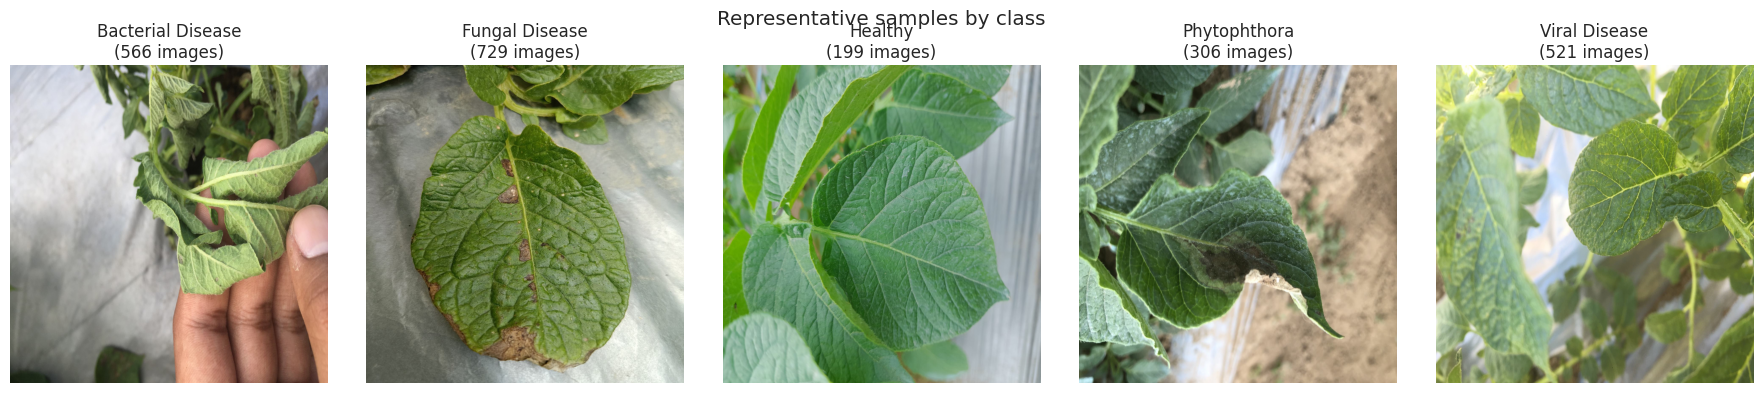
\includegraphics[width=0.98\textwidth]{image/dataset_samples.png}
\caption{Representative field leaf samples across the five potato classes from the Kaggle dataset audit ($N = 2,321$).}
\label{fig:samples}
\end{figure}

\subsubsection{Leak-Aware Stratified Group Split}
Perceptual difference hashing ($\text{dHash} \le 10$) found \textbf{2,283 distinct image groups} in the 2,321 images. It caught 38 near-duplicate clusters, so the same leaf cannot appear in two subsets. \texttt{StratifiedGroupKFold} then gave the same separate splits for all four models. Figure~\ref{fig:class_split} plots the split, and Table~\ref{tab:data_splits} gives the numbers per class.

\begin{figure}[!htbp]
\centering
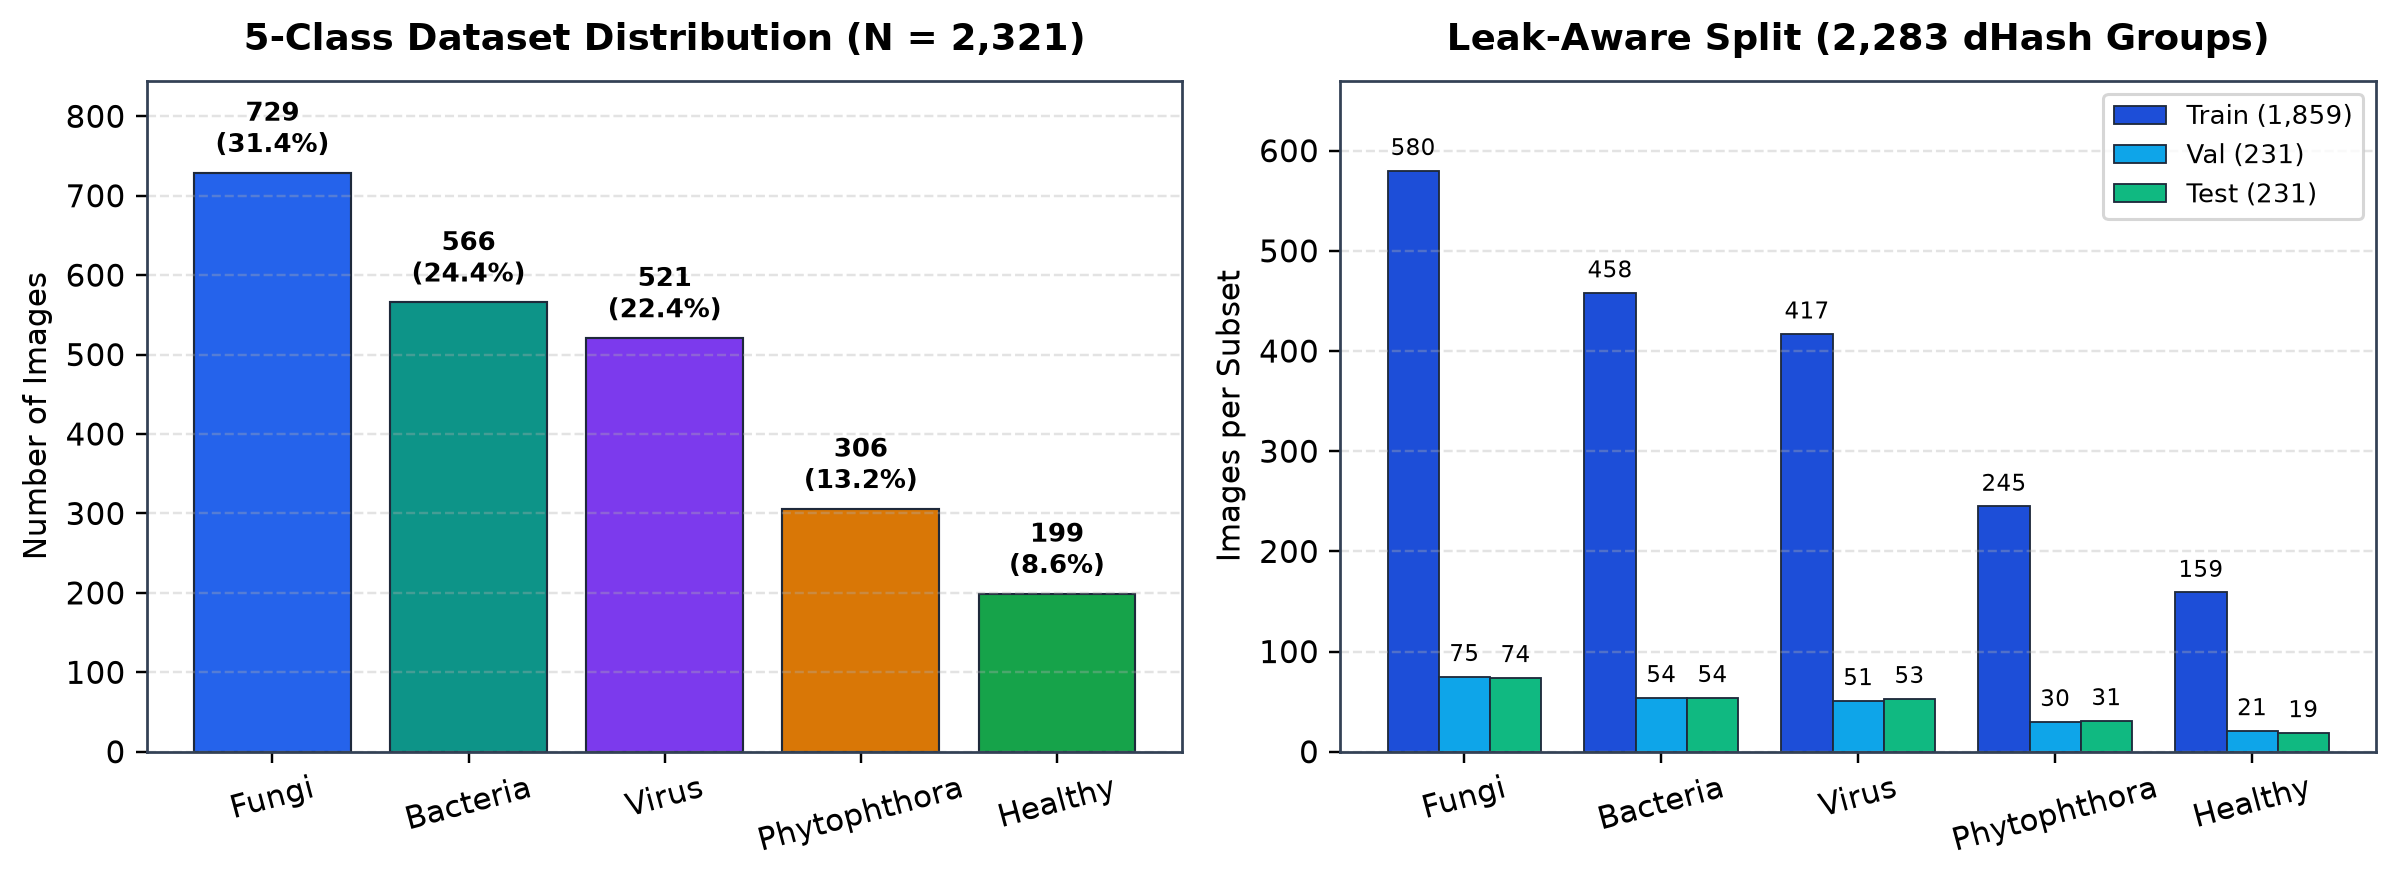
\includegraphics[width=0.96\textwidth]{image/class_split_dist.png}
\caption[Five-class dataset distribution and leak-aware data split.]{Five-class dataset distribution (left) and leak-aware Train/Validation/Test split across 2,283 perceptual-hash groups (right).}
\label{fig:class_split}
\end{figure}

\begin{table}[htbp]
\caption{Exact Per-Class Breakdown of the Leak-Aware 80:10:10 Split (Shared Across All 4 Architectures)}
\label{tab:data_splits}
\begin{center}
\setlength{\tabcolsep}{4pt}
\begin{tabularx}{\textwidth}{| >{\raggedright\arraybackslash}X | c | c | c | c | c |}
\hline
\textbf{Class (Display Name)} & \textbf{Train (80\%)} & \textbf{Val (10\%)} & \textbf{Test (10\%)} & \textbf{Total} & \textbf{Weight} \\
\hline
Bacteria (Bacterial Disease) & 458 & 54 & 54 & 566 & 0.6546 \\
\hline
Fungi (Fungal Disease) & 580 & 75 & 74 & 729 & 0.5169 \\
\hline
Healthy & 159 & 21 & 19 & 199 & 1.8857 \\
\hline
Phytopthora (Phytophthora) & 245 & 30 & 31 & 306 & 1.2238 \\
\hline
Virus (Viral Disease) & 417 & 51 & 53 & 521 & 0.7190 \\
\hline
\textbf{Total Images} & \textbf{1,859} & \textbf{231} & \textbf{231} & \textbf{2,321} & \textbf{Mean 1.00} \\
\hline
\end{tabularx}
\end{center}
\end{table}

\subsection{Model Implementation}
Table~\ref{tab:arch_specs} compares our MobileNetV2 with the three benchmark models: input size, parameters, weight size, head, learning rates and the Grad-CAM layer. Table~\ref{tab:mnv2_layers} lists the layers of our MobileNetV2 (2,264,389 parameters in total, 8.64~MB).

\begin{table}[htbp]
\caption{Architectural and Training Configuration Summary Across All Four Benchmarked Architectures}
\label{tab:arch_specs}
\begin{center}
\small
\setlength{\tabcolsep}{3.5pt}
\begin{tabularx}{\textwidth}{| L{2.6cm} | c | r | r | X | L{2.1cm} | L{1.9cm} |}
\hline
\textbf{Model} & \textbf{Input} & \textbf{Params} & \textbf{MB} & \textbf{Head Design} & \textbf{Head / FT LR} & \textbf{Grad-CAM Layer} \\
\hline
\textbf{Proposed MobileNetV2} & $224^2$ & \textbf{2.26M} & \textbf{8.64} & GAP $\rightarrow$ Drop(0.25) $\rightarrow$ Dense(5) & $10^{-3}$ / $10^{-4}$ (AdamW, BN frozen) & \texttt{Conv\_1} \\
\hline
NASNetMobile & $224^2$ & 4.54M & 17.33 & GAP $\rightarrow$ Dense(256) + BN + Swish $\rightarrow$ Dense(5) & $3\!\times\!10^{-4}$ / $3\!\times\!10^{-5}$ & \texttt{normal\_\allowbreak conv\_\allowbreak 1\_\allowbreak 12} \\
\hline
InceptionV3 & $299^2$ & 22.33M & 85.18 & GAP $\rightarrow$ Dense(256) + BN + Swish $\rightarrow$ Dense(5) & $3\!\times\!10^{-4}$ / $3\!\times\!10^{-5}$ & \texttt{conv2d\_93} \\
\hline
MultiNet-V3 Ensemble & $224^2$ & 31.08M & 118.55 & 3-Backbone Concat $\rightarrow$ GAP $\rightarrow$ Dense(256) $\rightarrow$ Dense(5) & $3\!\times\!10^{-4}$ / $3\!\times\!10^{-5}$ & \texttt{ensemble\_\allowbreak spatial\_\allowbreak features} \\
\hline
\end{tabularx}
\end{center}
\end{table}

\begin{table}[htbp]
\caption{Compact Topology and Parameter Breakdown of the Proposed MobileNetV2 Model}
\label{tab:mnv2_layers}
\begin{center}
\small
\setlength{\tabcolsep}{4pt}
\begin{tabularx}{\textwidth}{| L{4.1cm} | c | r | X |}
\hline
\textbf{Layer (Type)} & \textbf{Output Shape} & \textbf{Param \#} & \textbf{Role in Pipeline} \\
\hline
\texttt{image} (\texttt{InputLayer}) & $(224,224,3)$ & 0 & Normalized RGB input $[0, 1]$ (FastAPI contract) \\
\hline
\texttt{mobilenetv2\_\allowbreak preprocessing} (\texttt{Rescaling}) & $(224,224,3)$ & 0 & Native scaling $[0, 1] \rightarrow [-1, 1]$ \\
\hline
\texttt{mobilenetv2\_\allowbreak 1.00\_\allowbreak 224} (\texttt{Functional}) & $(7,7,1280)$ & 2,257,984 & 154-layer ImageNet backbone (top 54 non-BN unfrozen in Stage~2) \\
\hline
\texttt{global\_\allowbreak average\_\allowbreak pool} (\texttt{GAP2D}) & $(1280)$ & 0 & Spatial compression \& structural feature selector \\
\hline
\texttt{dropout\_\allowbreak features} (\texttt{Dropout}) & $(1280)$ & 0 & Regularization ($p = 0.25$) \\
\hline
\texttt{classifier} (\texttt{Dense}, Softmax) & $(5)$ & 6,405 & 5-class probability distribution \\
\hline
\textbf{Total Parameters} & & \textbf{2,264,389} & \textbf{8.64~MB} (Stage~1: 6,405 trainable; Stage~2: 36 non-BN layers + head) \\
\hline
\end{tabularx}
\end{center}
\end{table}

\subsection{Evaluation Metrics}
Every model is tested on the same $N = 231$ unseen images in $C = 5$ classes. We use the usual multi-class metrics \cite{grandini2020metrics}, plus an export check and a size-efficiency measure:
\begin{itemize}
    \item \textbf{Label-smoothed categorical cross-entropy loss.} With soft targets $y^{\text{LS}}_k = (1 - \epsilon) y_k + \frac{\epsilon}{C}$ ($\epsilon = 0.05$ in our proposed recipe; $\epsilon = 0.10$ in benchmarks):
    \begin{equation}
    \mathcal{L} = -\sum_{k=1}^{C} y^{\text{LS}}_k \log(\hat{p}_k).
    \end{equation}
    \item \textbf{Accuracy, per-class precision, recall and F1, and macro-F1.}
    \begin{equation}
    \begin{aligned}
    \text{Accuracy} &= \frac{\sum_{k=1}^{C} \text{TP}_k}{N}, \qquad
    \text{F1}_k = \frac{2\,\text{TP}_k}{2\,\text{TP}_k + \text{FP}_k + \text{FN}_k}, \\
    \text{Macro-F1} &= \frac{1}{C} \sum_{k=1}^{C} \text{F1}_k.
    \end{aligned}
    \end{equation}
    Macro-F1 gives the five classes equal weight, whatever their size. A model that favors the largest class is therefore penalized.
    \item \textbf{Export difference.} $\Delta_{\max} = \max_{i,k} |\hat{p}^{\text{reloaded}}_{i,k} - \hat{p}^{\text{selected}}_{i,k}|$ must be $\Delta_{\max} \le 10^{-3}$. All models passed with $\Delta_{\max} = 0.00 \times 10^{0}$.
    \item \textbf{Accuracy against size, and Pareto fronts.} To measure size together with accuracy, we find the non-dominated Pareto fronts over $(\text{Macro-F1}, \text{Size in MB})$. We also report the log-scale ratio $\eta = \text{Macro-F1} / \log_{10}(\text{Size}_{\text{MB}})$.
\end{itemize}

\subsection{Performance Analysis}

\subsubsection{Proposed MobileNetV2 Results and Fine-Tuning Optimization Ablation}
Before we fixed the final model, we ran an ablation on the training setup. The architecture stayed the same in both runs (8.64~MB MobileNetV2, 2,264,389 parameters). The first run was our baseline: the top 30 layers unfrozen, Batch Normalization included, Adam, 40 epochs and geometric augmentation only. The second run used the optimized setup: restoring the best Stage~1 weights, the top 54 layers unfrozen with BN kept frozen, AdamW with weight decay $10^{-4}$ and gradient clipping, vertical flips plus brightness and shear augmentation, up to 60 epochs, and optional 4-view TTA.

In the baseline, the BN layers were unfrozen at Epoch~9. The validation loss jumped from $0.8344$ to $2.6258$, and validation macro-F1 fell from $0.7918$ to $0.4356$. The model needed about 12 epochs to recover. At Epoch~40 it reached 91.34\% test accuracy (0.9119 macro-F1), and it was still improving when training ended. The optimized run is shown in Figure~\ref{fig:02_curves}. Here we restored the Epoch~6 head checkpoint (\texttt{val\_macro\_f1 = 0.8085}) and kept all BN layers frozen, and the fine-tuning shock did not happen. At Epoch~11 the validation loss went down ($0.7007 \rightarrow 0.6955$) instead of up. Validation macro-F1 rose steadily to a peak of \textbf{0.9184} at Epoch~33 (92.21\% validation accuracy, \texttt{val\_loss = 0.4434}), and Early Stopping ended the run at Epoch~45.

\begin{figure}[!htbp]
\centering
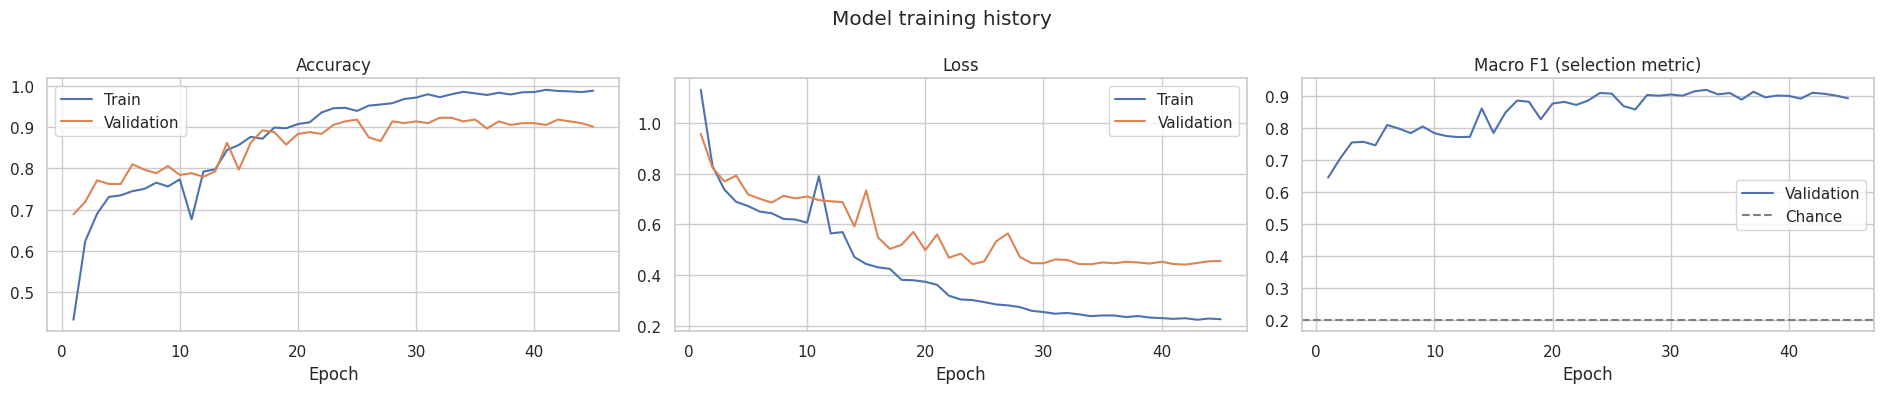
\includegraphics[width=0.98\textwidth]{image/training_curves.png}
\caption[Training and validation curves for Proposed MobileNetV2.]{Training and validation accuracy, loss, and macro-F1 curves for the proposed fine-tuned MobileNetV2 model (45 epochs; no fine-tuning shock when Stage~2 starts).}
\label{fig:02_curves}
\end{figure}

Table~\ref{tab:ft_ablation} sums up the effect. The changes add no parameters, yet single-pass test accuracy rose from \textbf{91.34\% to 93.51\%} ($+2.17$ percentage points). Macro-F1 rose from \textbf{0.9119 to 0.9272} ($+0.0153$), and test loss fell by 33.6\% ($0.6727 \rightarrow 0.4466$). With 4-view TTA on the same exported file (\texttt{explainable\_\allowbreak cnn\_\allowbreak model.keras}), the scores went up again to \textbf{93.94\% accuracy} and \textbf{0.9317 macro-F1}. Table~\ref{tab:02_per_class} and the confusion matrix in Figure~\ref{fig:02_cm} give the per-class picture. Recall is \textbf{100\%} for both \textit{Bacterial Disease} (54/54, F1~0.99) and \textit{Healthy} (19/19). \textit{Viral Disease} reaches \textbf{0.96 F1} (0.98 precision). For \textit{Phytophthora}, the hardest disease class, recall went up by 13 percentage points ($0.81 \rightarrow 0.94$, F1~0.89).

\begin{table}[htbp]
\caption{Zero-Size-Cost Training Optimization Ablation on Proposed MobileNetV2 ($N = 231$)}
\label{tab:ft_ablation}
\begin{center}
\begin{tabularx}{\textwidth}{| X | c | c | c | c | c |}
\hline
\textbf{Training Configuration (All 2.26M Params / 8.64~MB)} & \textbf{Epochs} & \textbf{Test Loss} & \textbf{Test Acc (\%)} & \textbf{Macro-F1} & \textbf{Mean Conf.} \\
\hline
Baseline MobileNetV2 (Adam, unfrozen BN, 30 layers) & 40 & 0.6727 & 91.34\% & 0.9119 & 0.8831 \\
\hline
\textbf{Proposed MobileNetV2 (AdamW, frozen BN, 54 layers)} & \textbf{45 (ES)} & \textbf{0.4466} & \textbf{93.51\%} & \textbf{0.9272} & \textbf{0.9016} \\
\hline
\textbf{Proposed MobileNetV2 + 4-View TTA (same file)} & \textbf{45 (ES)} & --- & \textbf{93.94\%} & \textbf{0.9317} & --- \\
\hline
\end{tabularx}
\end{center}
\end{table}

\begin{table}[htbp]
\caption{Detailed Per-Class Classification Report of Proposed MobileNetV2 (Single-Pass, $N = 231$)}
\label{tab:02_per_class}
\begin{center}
\begin{tabularx}{\textwidth}{| X | c | c | c | c |}
\hline
\textbf{Class} & \textbf{Precision} & \textbf{Recall} & \textbf{F1-Score} & \textbf{Support} \\
\hline
Bacterial Disease & 0.98 & 1.00 & 0.99 & 54 \\
\hline
Fungal Disease & 0.96 & 0.86 & 0.91 & 74 \\
\hline
Healthy & 0.79 & 1.00 & 0.88 & 19 \\
\hline
Phytophthora & 0.85 & 0.94 & 0.89 & 31 \\
\hline
Viral Disease & 0.98 & 0.94 & 0.96 & 53 \\
\hline
\textbf{Overall Accuracy / Macro Avg} & \textbf{0.91} & \textbf{0.95} & \textbf{0.93 (0.9272)} & \textbf{231} \\
\hline
\textbf{Weighted Average} & \textbf{0.94} & \textbf{0.94} & \textbf{0.94} & \textbf{231} \\
\hline
\end{tabularx}
\end{center}
\end{table}

\begin{figure}[!htbp]
\centering
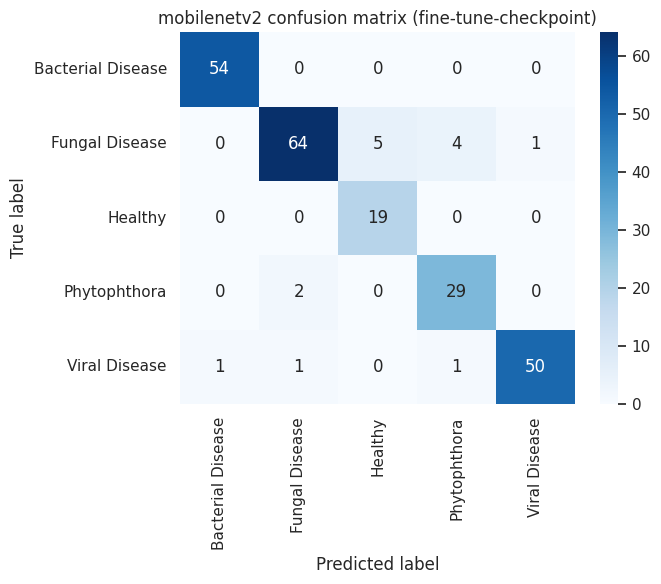
\includegraphics[width=0.68\textwidth]{image/confusion_matrix.png}
\caption[Confusion matrix of Proposed MobileNetV2 on the 231-image test set.]{Confusion matrix of the proposed fine-tuned MobileNetV2 (\texttt{fine-tune-checkpoint}) on the 231-image leak-aware test set (93.51\% accuracy, 0.9272 macro-F1).}
\label{fig:02_cm}
\end{figure}

\FloatBarrier
\subsubsection{MultiNet-V3 Ensemble Benchmark Results}
MultiNet-V3 (EfficientNetB0 + MobileNetV2 + ResNet50, 31.08M parameters, 118.55~MB) is our large ensemble reference. Stage~1 reached \texttt{val\_macro\_f1 = 0.8866} quickly, by Epoch~5. Stage~2 peaked at \texttt{val\_macro\_f1 = 0.9152} (91.77\% validation accuracy) at Epoch~16, and Early Stopping ended training at Epoch~24 (Figure~\ref{fig:multinet_curves}). On the 231 test images, the chosen \texttt{final-epoch} checkpoint scored \textbf{90.91\% accuracy}, \textbf{0.8975 macro-F1} and \textbf{0.6853 test loss}, with a mean confidence of 0.8679 (Figure~\ref{fig:multinet_cm}). MultiNet-V3 did well on Bacterial (0.96 F1, 100\% recall) and Phytophthora (0.89 F1). But it gave false positives for \textit{Healthy}, the smallest class: some diseased leaves were labeled healthy (0.70 precision, 0.83 F1). It also needs $13.7\times$ more storage than our MobileNetV2, and its accuracy is 2.60 percentage points lower.

\begin{figure}[H]
\centering
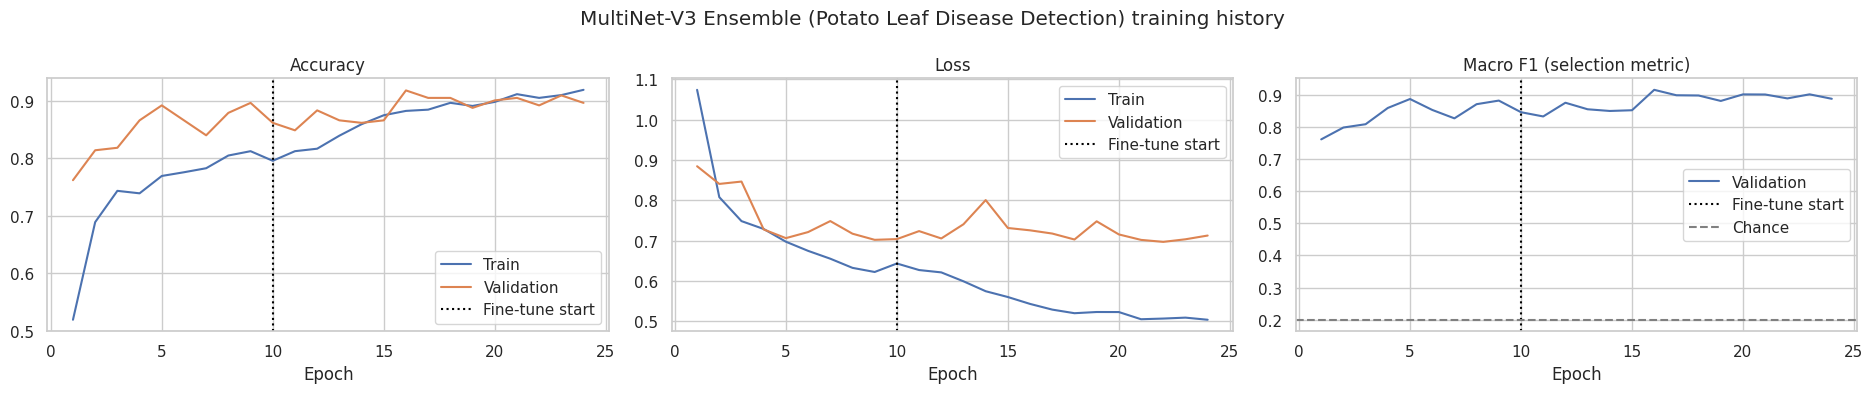
\includegraphics[width=0.98\textwidth]{image/multinet_training_curves.png}
\caption{Training and validation learning curves for the MultiNet-V3 Ensemble benchmark (24 epochs, early stopped).}
\label{fig:multinet_curves}
\end{figure}

\begin{figure}[H]
\centering
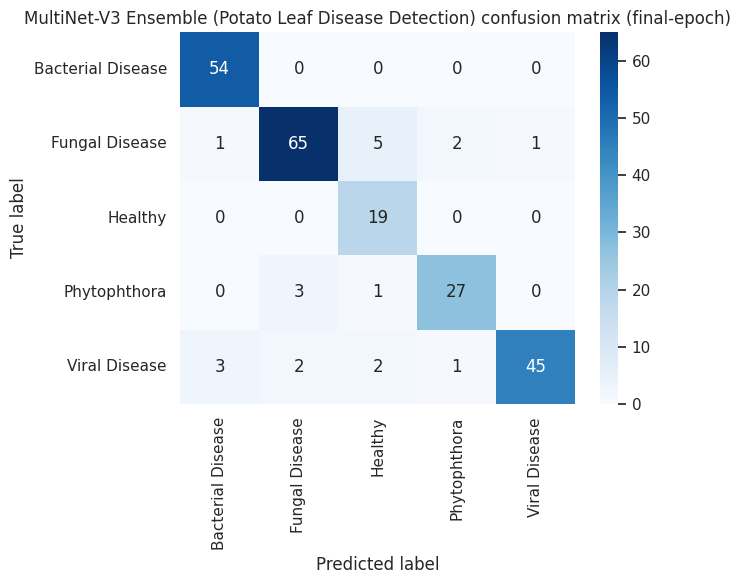
\includegraphics[width=0.55\textwidth]{image/multinet_confusion_matrix.png}
\caption{Confusion matrix of the MultiNet-V3 Ensemble benchmark on the 231-image test set (90.91\% accuracy, 0.8975 macro-F1).}
\label{fig:multinet_cm}
\end{figure}

Figure~\ref{fig:multinet_curves} has three panels: accuracy, loss and validation macro-F1 for each epoch. The dotted line at Epoch~10 marks the start of fine-tuning. The training loss keeps going down, but the validation loss stays around 0.7 after Epoch~5, so the model gains little from the later epochs. In the confusion matrix (Figure~\ref{fig:multinet_cm}), each row is the true class and each column is the predicted class, so the correct answers are on the diagonal. All 54 Bacterial leaves are correct. Most errors are diseased leaves that were labeled \textit{Healthy}: 5 Fungal, 1 Phytophthora and 2 Viral leaves. This explains the low \textit{Healthy} precision.

\FloatBarrier
\subsubsection{InceptionV3 Benchmark Results}
InceptionV3 (22.33M parameters, 85.18~MB, $299 \times 299$ input) trained for 33 epochs before Early Stopping. Its best \texttt{val\_macro\_f1} was 0.8508, at Epoch~25 (Figure~\ref{fig:inception_curves}). On the 231 test images it scored \textbf{84.42\% accuracy}, \textbf{0.8296 macro-F1} and \textbf{0.7353 test loss} (Figure~\ref{fig:inception_cm}). It reached 0.96 F1 on Bacterial Disease. Its Fungal recall (0.73), Phytophthora F1 (0.72) and Healthy precision (0.63), however, were all below our MobileNetV2, even though InceptionV3 needs $9.86\times$ more storage and $1.78\times$ more input pixels per image.

\begin{figure}[!htbp]
\centering
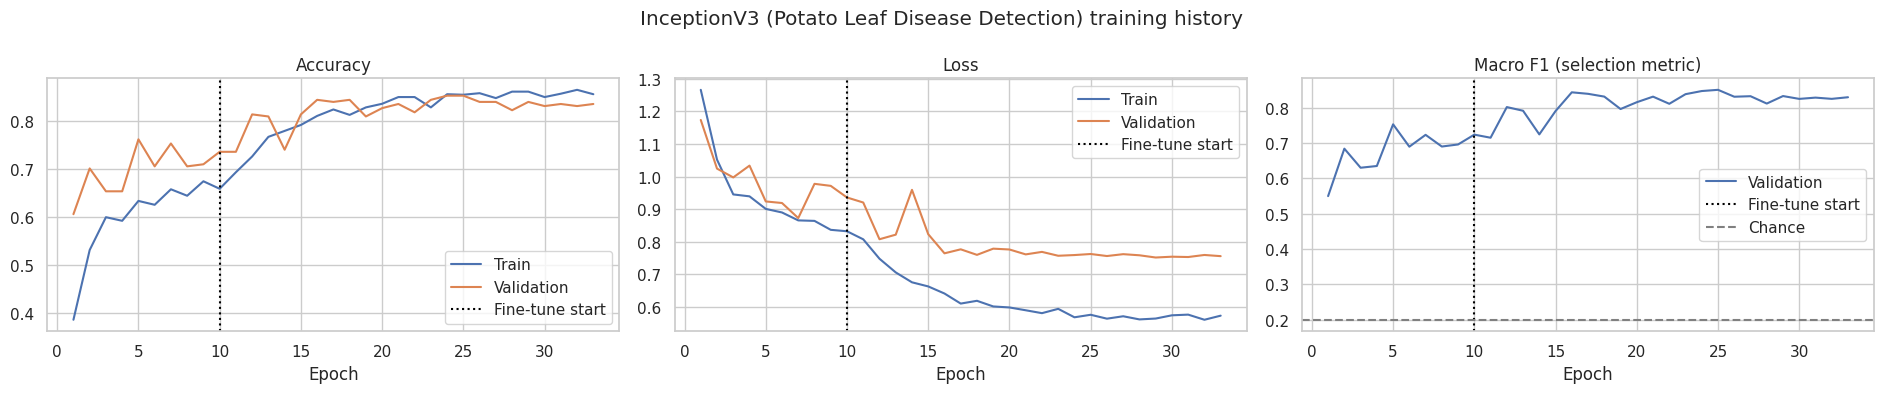
\includegraphics[width=0.98\textwidth]{image/inception_training_curves.png}
\caption{Training and validation learning curves for the InceptionV3 ($299 \times 299$) benchmark (33 epochs).}
\label{fig:inception_curves}
\end{figure}

\begin{figure}[!htbp]
\centering
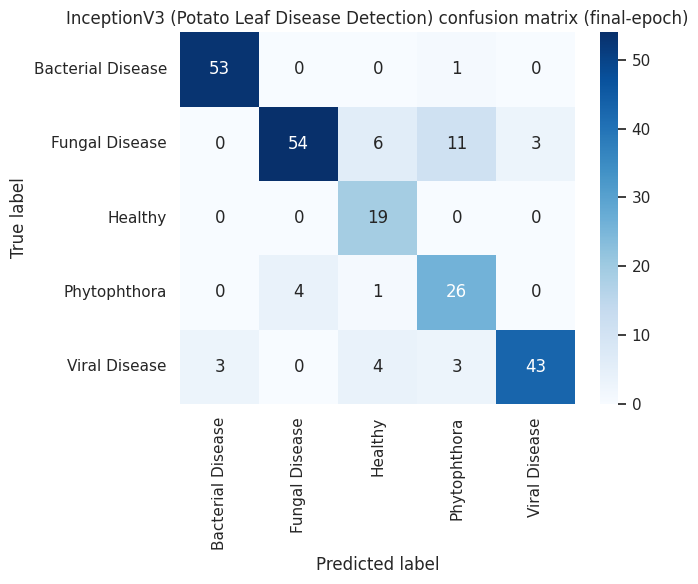
\includegraphics[width=0.55\textwidth]{image/inception_confusion_matrix.png}
\caption{Confusion matrix of InceptionV3 on the 231-image test set (84.42\% accuracy, 0.8296 macro-F1).}
\label{fig:inception_cm}
\end{figure}

Figures~\ref{fig:inception_curves} and~\ref{fig:inception_cm} use the same layout as the MultiNet-V3 figures. The curves show accuracy, loss and validation macro-F1 for each epoch, and the dotted line marks the start of fine-tuning. In the confusion matrix, the rows are the true classes, the columns are the predicted classes and the correct answers are on the diagonal.

\FloatBarrier
\subsubsection{NASNetMobile Benchmark Results}
NASNetMobile (4.54M parameters, 17.33~MB) did not adapt well. Its searched cells have many branches, and our dataset is only medium-sized. Validation macro-F1 peaked at 0.6964 at Epoch~13, and training stopped early at Epoch~21 (Figure~\ref{fig:nasnet_curves}). On the unseen test set it scored \textbf{72.73\% accuracy}, \textbf{0.7049 macro-F1} and \textbf{0.9642 test loss}, with a mean confidence of 0.6633 (Figure~\ref{fig:nasnet_cm}). It confused many leaves in Healthy (0.40 precision, 0.54 F1), Phytophthora (0.63 F1) and Fungal Disease (0.58 recall).

\begin{figure}[!htbp]
\centering
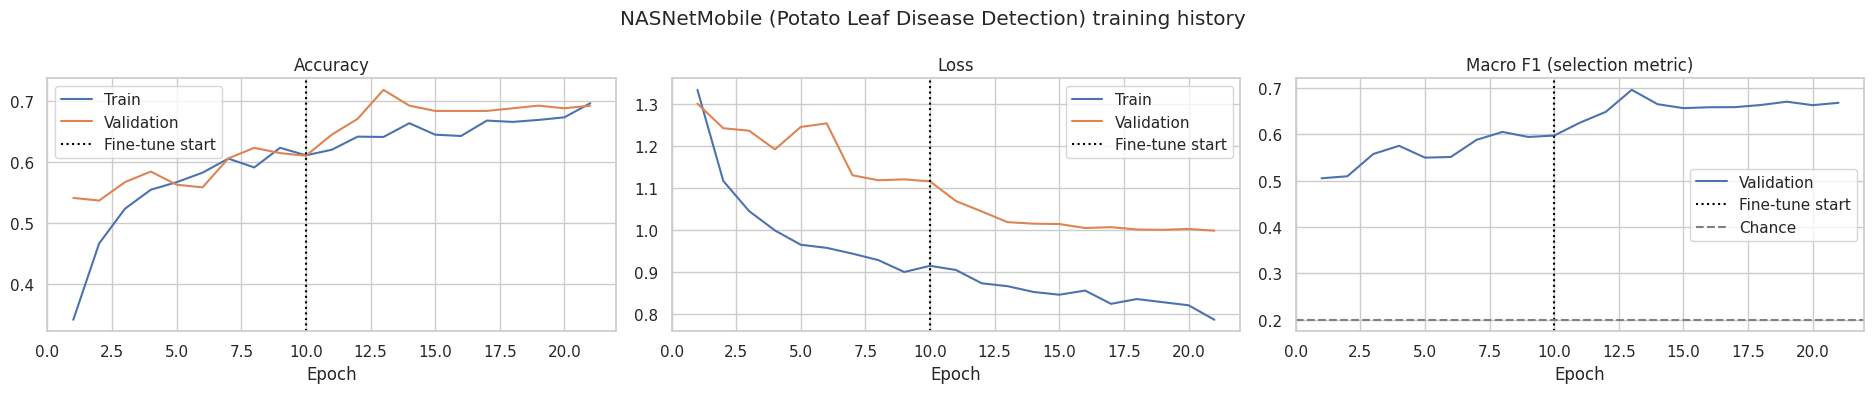
\includegraphics[width=0.98\textwidth]{image/nasnet_training_curves.png}
\caption{Training and validation learning curves for the NASNetMobile benchmark (21 epochs, early stopped).}
\label{fig:nasnet_curves}
\end{figure}

\begin{figure}[!htbp]
\centering
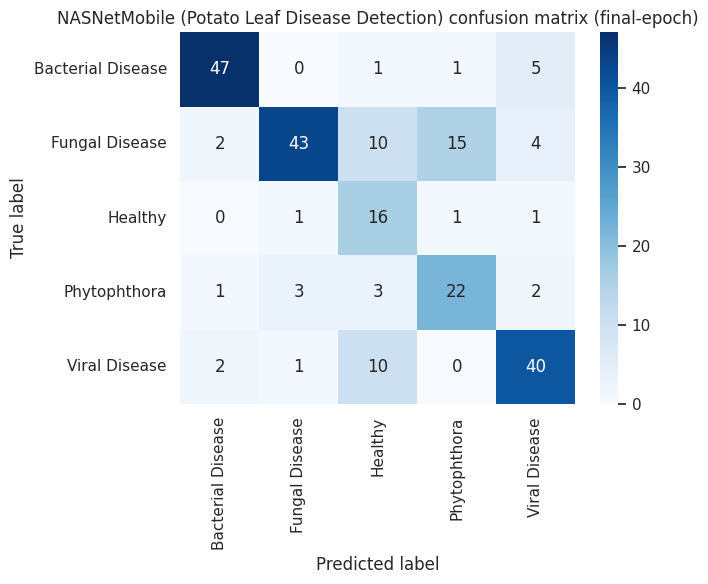
\includegraphics[width=0.55\textwidth]{image/nasnet_confusion_matrix.png}
\caption{Confusion matrix of NASNetMobile on the 231-image test set (72.73\% accuracy, 0.7049 macro-F1).}
\label{fig:nasnet_cm}
\end{figure}

Figures~\ref{fig:nasnet_curves} and~\ref{fig:nasnet_cm} again use the same layout. Here the numbers off the diagonal of the confusion matrix are much larger than for the other models, which matches the low accuracy and the weak \textit{Healthy}, \textit{Phytophthora} and \textit{Fungal} scores.

\FloatBarrier
\subsection{Key Findings and Discussions}

\subsubsection{Comparison of All Models and Accuracy-to-Size Analysis}
Table~\ref{tab:final_summary} ranks the four models by Pareto accuracy-to-size dominance on the same 231-image test split. Table~\ref{tab:per_class_all} gives the per-class F1 of each model. Figure~\ref{fig:bench_comp} shows overall and per-class results side by side, and Figure~\ref{fig:pareto} plots the accuracy-to-size Pareto frontier on a log scale.

\begin{table}[htbp]
\caption{Master Benchmark Comparison Ordered by Accuracy-to-Size Pareto Dominance ($N = 231$)}
\label{tab:final_summary}
\begin{center}
\small
\setlength{\tabcolsep}{3.5pt}
\begin{tabularx}{\textwidth}{| c | X | r | r | c | c | c | c | c |}
\hline
\textbf{\#} & \textbf{Model} & \textbf{Params} & \textbf{MB} & \textbf{Loss} & \textbf{Acc} & \textbf{Macro-F1} & \textbf{F1/$\log$MB} & \textbf{Pareto} \\
\hline
\textbf{1} & \textbf{Proposed MobileNetV2 (4-View TTA)} & \textbf{2.26M} & \textbf{8.64} & --- & \textbf{93.94\%} & \textbf{0.9317} & \textbf{0.995} & \textbf{Front 1} \\
\hline
\textbf{1} & \textbf{Proposed MobileNetV2 (Single-Pass)} & \textbf{2.26M} & \textbf{8.64} & \textbf{0.4466} & \textbf{93.51\%} & \textbf{0.9272} & \textbf{0.990} & \textbf{Front 1} \\
\hline
2 & MultiNet-V3 Ensemble (3 Backbones) & 31.08M & 118.55 & 0.6853 & 90.91\% & 0.8975 & 0.433 & Front 2 \\
\hline
3 & InceptionV3 ($299 \times 299$) & 22.33M & 85.18 & 0.7353 & 84.42\% & 0.8296 & 0.430 & Front 2 \\
\hline
4 & NASNetMobile & 4.54M & 17.33 & 0.9642 & 72.73\% & 0.7049 & 0.569 & Front 2 \\
\hline
\end{tabularx}
\end{center}
\end{table}

\begin{table}[htbp]
\caption{Per-Class Test F1-Score Comparison Across All Four Benchmarked Architectures (Single-Pass, $N = 231$)}
\label{tab:per_class_all}
\begin{center}
\setlength{\tabcolsep}{4pt}
\begin{tabularx}{\textwidth}{| >{\raggedright\arraybackslash}X | c | c | c | c |}
\hline
\textbf{Class (Support)} & \textbf{Proposed MobileNetV2} & \textbf{MultiNet-V3} & \textbf{InceptionV3} & \textbf{NASNetMobile} \\
\hline
Bacterial Disease (54) & \textbf{0.99} & 0.96 & 0.96 & 0.89 \\
\hline
Fungal Disease (74) & \textbf{0.91} & 0.90 & 0.82 & 0.70 \\
\hline
Healthy (19) & \textbf{0.88} & 0.83 & 0.78 & 0.54 \\
\hline
Phytophthora (31) & \textbf{0.89} & \textbf{0.89} & 0.72 & 0.63 \\
\hline
Viral Disease (53) & \textbf{0.96} & 0.91 & 0.87 & 0.76 \\
\hline
\textbf{Macro-Average F1} & \textbf{0.9272} & 0.8975 & 0.8296 & 0.7049 \\
\hline
\end{tabularx}
\end{center}
\end{table}

\begin{figure}[H]
\centering
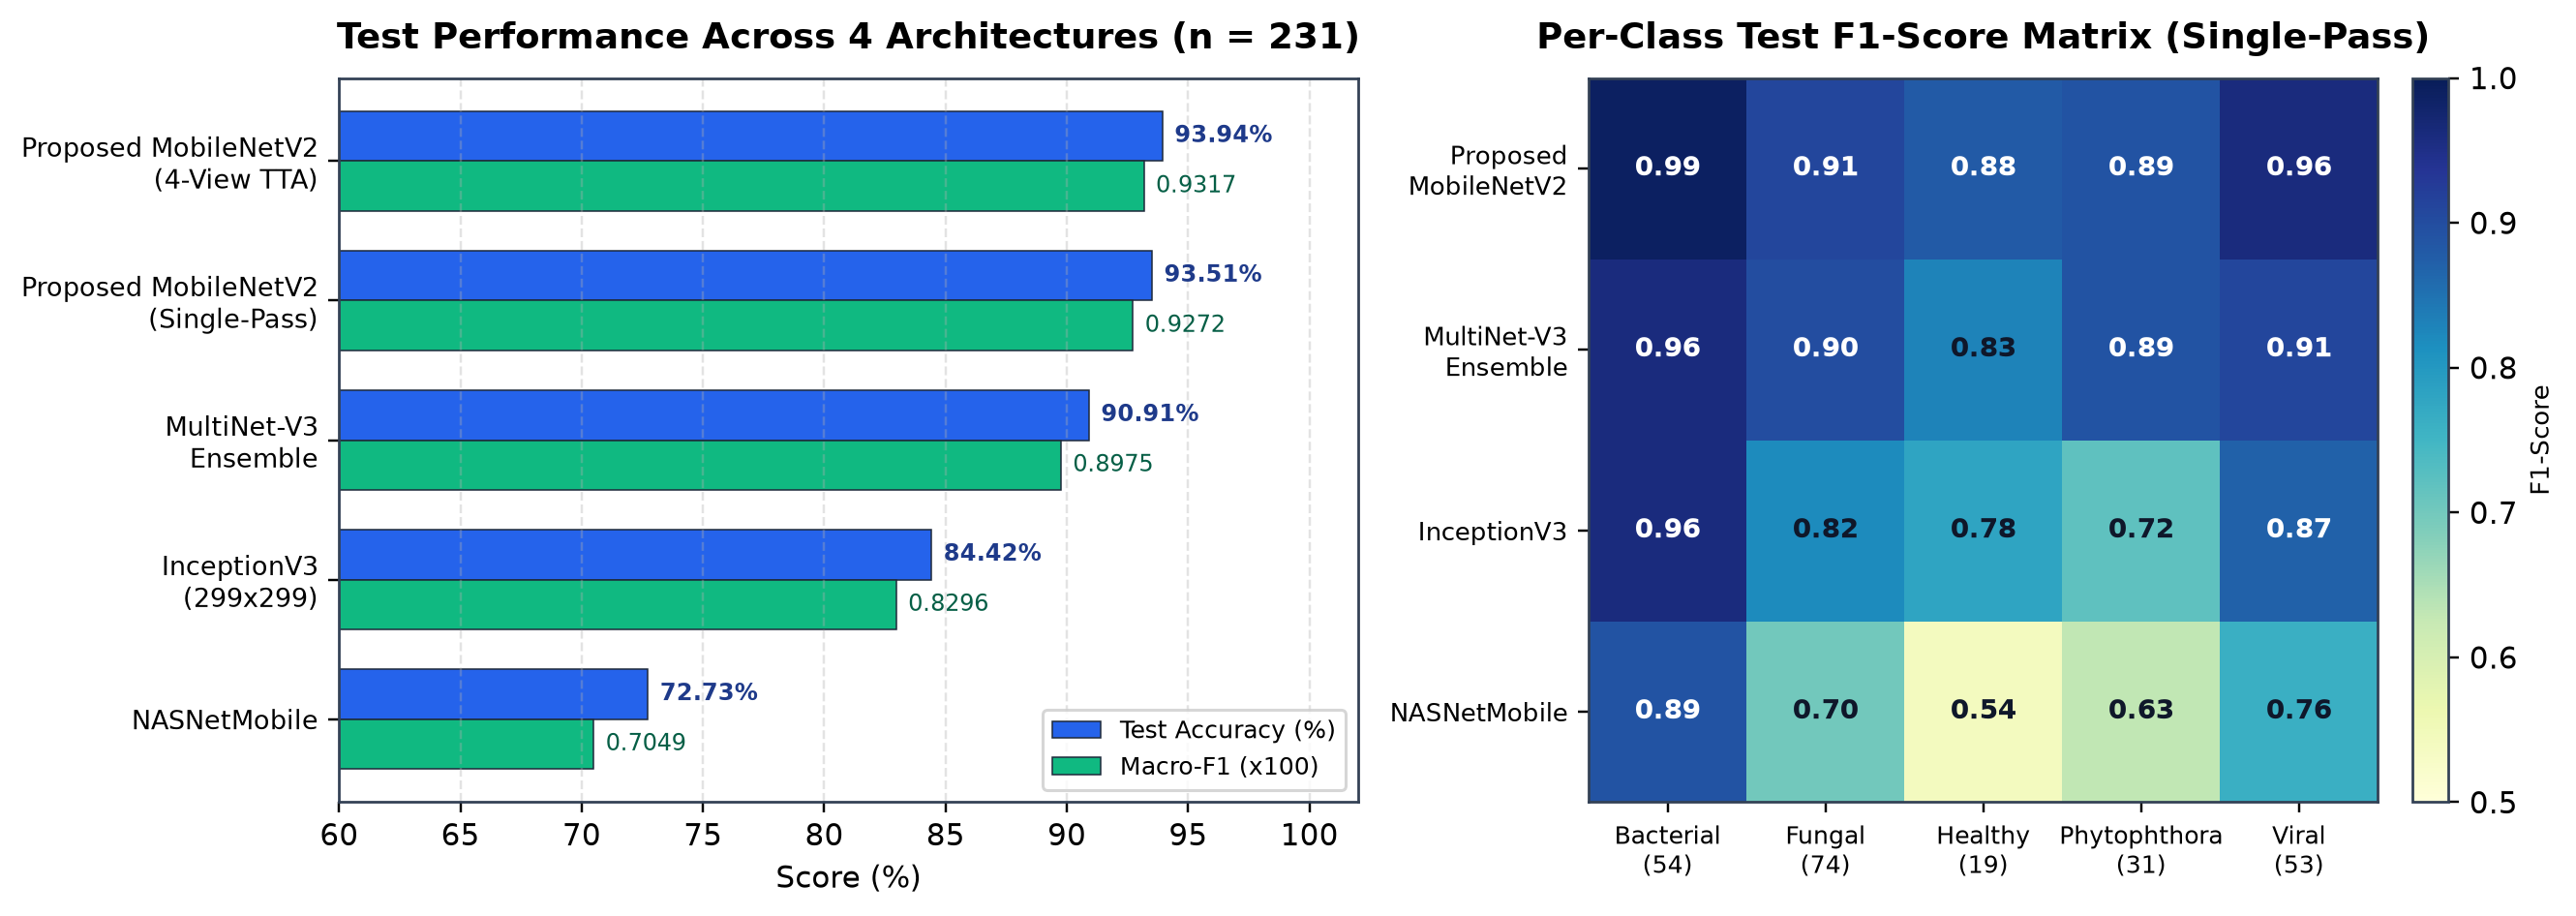
\includegraphics[width=0.9\textwidth]{image/benchmark_comparison.png}
\caption{Overall test accuracy and macro-F1 across all four benchmarked architectures (left) and per-class F1 heatmap (right) on the identical 231-image leak-aware test split.}
\label{fig:bench_comp}
\end{figure}

\begin{figure}[H]
\centering
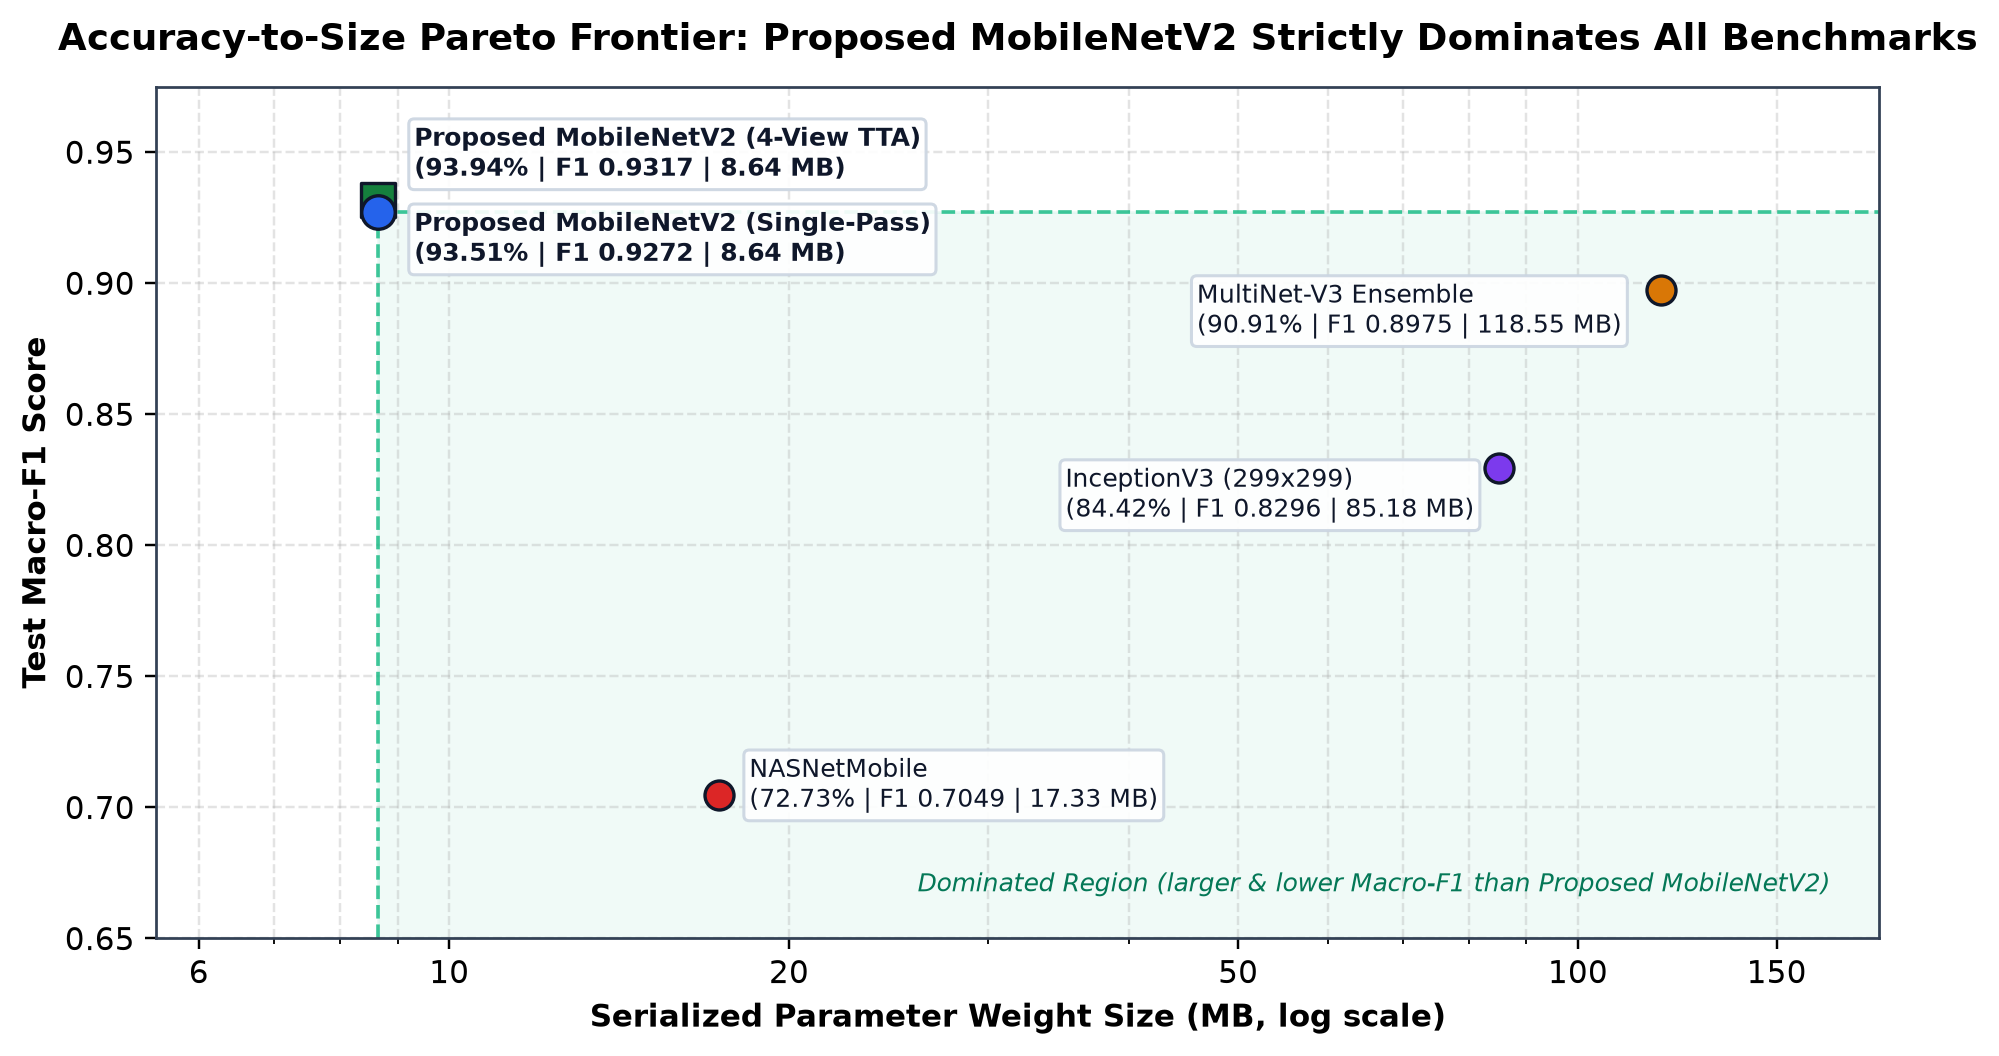
\includegraphics[width=0.8\textwidth]{image/pareto_tradeoff.png}
\caption{Accuracy-to-size Pareto frontier (Test Macro-F1 vs.\ serialized weight size in MB on a logarithmic scale). Proposed MobileNetV2 is the only model on Pareto Front~1; it is both smaller and more accurate than every other benchmark model.}
\label{fig:pareto}
\end{figure}

In Figure~\ref{fig:bench_comp}, the left chart shows a blue bar (test accuracy) and a green bar (macro-F1) for each model, from the best model at the top to the weakest at the bottom. The right chart is a heatmap of the F1-score for each class; darker blue means a higher score. The row of our MobileNetV2 is the darkest in every column. In Figure~\ref{fig:pareto}, each dot is one model. The x-axis is the file size in MB on a log scale, and the y-axis is the test macro-F1. A good model sits in the top-left corner: small and accurate. Our two MobileNetV2 points are in that corner, and the other three models are all to the right and lower, in the shaded area.

We draw four main points from this benchmark.

First, our MobileNetV2 is on the Pareto front by itself. At \textbf{8.64~MB} (2.26M parameters) it is both the \textbf{smallest} and the \textbf{most accurate} model we tested (93.51\% single-pass, 93.94\% with TTA; efficiency $0.990$--$0.995\;\text{F1}/\log_{10}\text{MB}$). MultiNet-V3 is $13.7\times$ larger and 2.60 percentage points less accurate. InceptionV3 is $9.9\times$ larger and 9.09 points less accurate. NASNetMobile is $2.0\times$ larger and 20.78 points less accurate.

Second, on a small field dataset the training setup mattered more than the parameter count. With 1,859 training images, neither stacking three heavy backbones (MultiNet-V3) nor raising the input to $299 \times 299$ (InceptionV3) beat a plain 6,405-parameter linear head trained with frozen-BN AdamW fine-tuning and leaf-like color augmentation.

Third, our model is at least as good as every other model on \textbf{all five classes}: Bacterial 0.99 vs.\ 0.96, Viral 0.96 vs.\ 0.91, Fungal 0.91 vs.\ 0.90, Phytophthora 0.89 vs.\ 0.89 and Healthy 0.88 vs.\ 0.83. The heavier models had poor precision on \textit{Healthy} (0.40--0.70). Our model reached 0.79.

Fourth, the exported models are safe to serve. When we reloaded each \texttt{.keras} file outside \texttt{MirroredStrategy}, the maximum probability difference was $0.00 \times 10^{0}$ for all four models. This means the file handed to the FastAPI backend behaves exactly like the trained model.

\subsubsection{Explainable AI (Grad-CAM) Validation Results}
Figures~\ref{fig:02_gradcam}, \ref{fig:multinet_gradcam} and \ref{fig:inception_gradcam} show Grad-CAM maps made from the trained Kaggle checkpoints on held-out test leaves. The layers are \texttt{Conv\_1} for our MobileNetV2, \texttt{ensemble\_\allowbreak spatial\_\allowbreak features} for MultiNet-V3 and \texttt{conv2d\_93} for InceptionV3. Each figure has three columns: the original leaf on the left, the heatmap in the middle and the heatmap laid over the leaf on the right. Red and yellow areas are the parts the model used most. Untrained or collapsed models tend to light up the image borders. The fine-tuned MobileNetV2 instead focuses on the diseased tissue: dark lesions, yellow mottling and blight edges. Soil and plastic mulch in the background get little attention. Single hard cases are also useful. In one example, a \textit{Viral Disease} leaf that looks unclear was predicted as \textit{Phytophthora} with 66.7\% confidence, and its heatmap moved partly onto the soil. A case like this shows how the heatmap and the confidence score together can warn the farmer to ask an expert when symptoms overlap.

\subsubsection{LLM-Based Advisory Pipeline}
Figure~\ref{fig:llm_pipeline} shows how the classifier output reaches Gemini. The figure is a flow chart with six steps from top to bottom: the leaf image, resizing to $224 \times 224$ and rescaling by 1/255, the CNN prediction (class and confidence), the prompt builder (7 topics and the safety rules), the Gemini API and, last, the advice text for the farmer. After the CNN predicts a disease and a softmax confidence, only these two fields are sent to Google Gemini (\texttt{gemini-3.1-flash-lite}). The user's photo is never sent. Gemini follows fixed safety rules. It explains the visible symptoms and sums up practical field and hygiene steps. It may not invent pesticide brands or doses. When confidence is low, it tells the farmer to contact the local agricultural extension officer.

\begin{figure}[H]
\centering
\captionsetup{font=small}
\begin{minipage}[t]{0.48\textwidth}
\centering
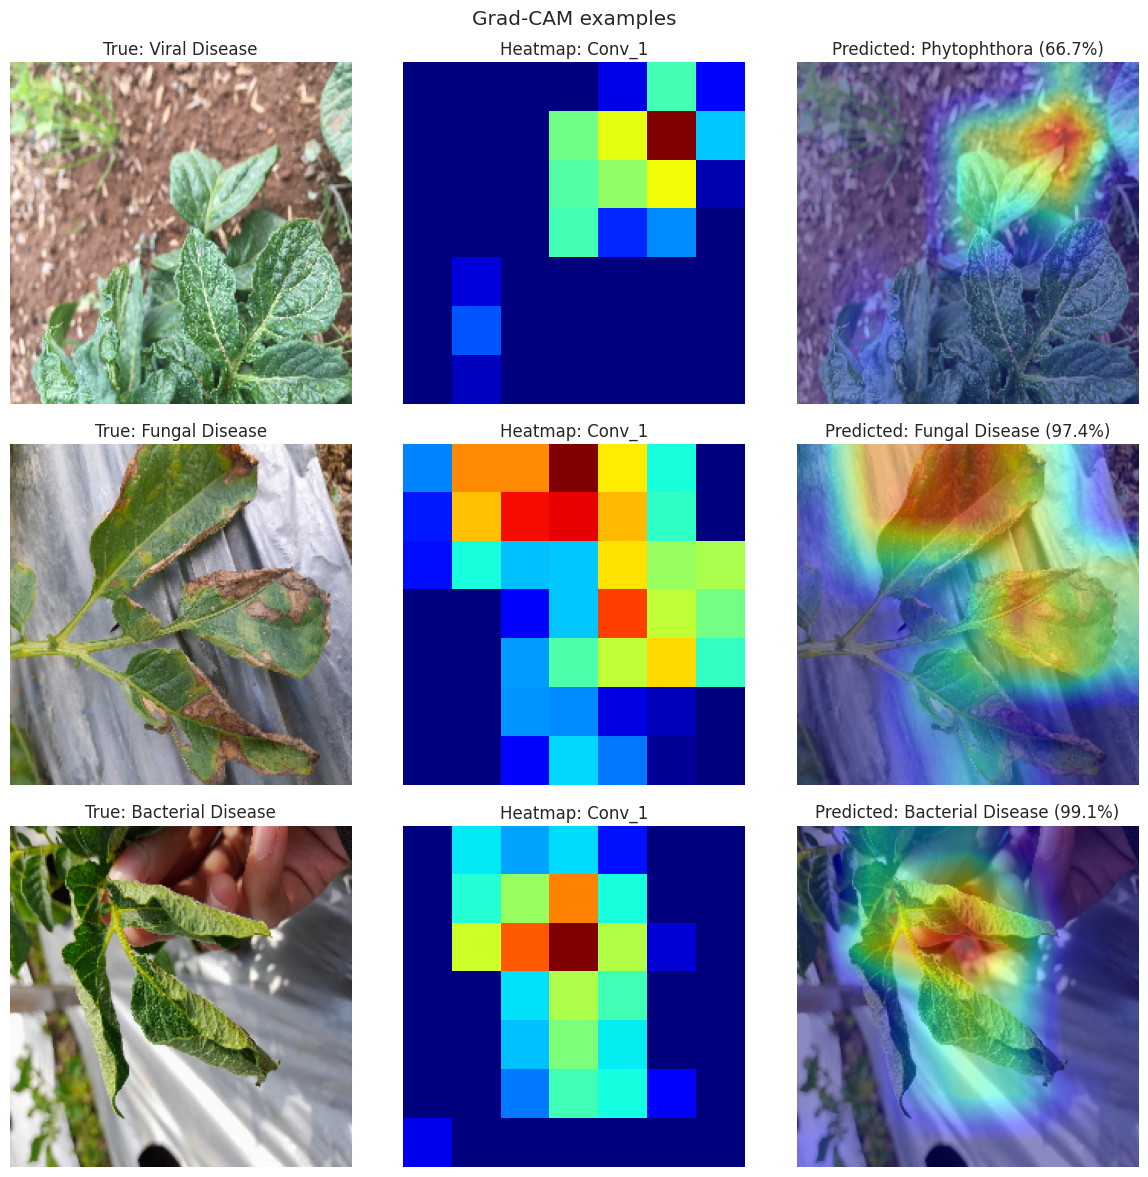
\includegraphics[width=\linewidth,height=5.4cm,keepaspectratio]{image/gradcam.png}
\captionof{figure}[Grad-CAM visual explanations from Proposed MobileNetV2.]{Grad-CAM from the proposed MobileNetV2 (\texttt{Conv\_1}): original image, heatmap and overlay on unseen test leaves.}
\label{fig:02_gradcam}
\end{minipage}\hfill
\begin{minipage}[t]{0.48\textwidth}
\centering
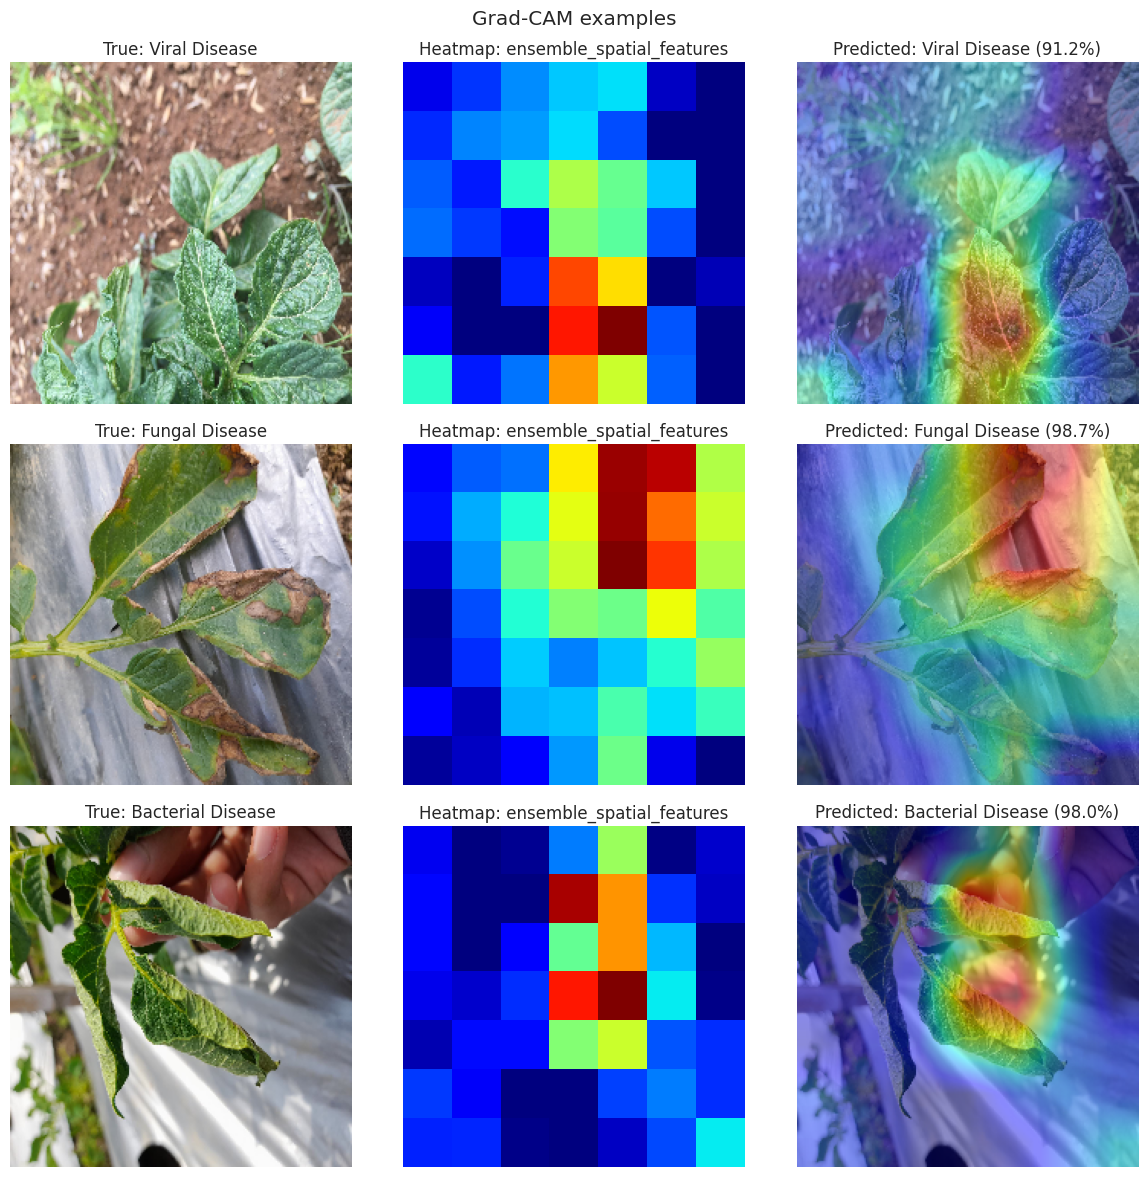
\includegraphics[width=\linewidth,height=5.4cm,keepaspectratio]{image/multinet_gradcam.png}
\captionof{figure}[Grad-CAM visual explanations from MultiNet-V3 Ensemble.]{Grad-CAM from the MultiNet-V3 Ensemble (\texttt{ensemble\_\allowbreak spatial\_\allowbreak features}) on the same test leaves.}
\label{fig:multinet_gradcam}
\end{minipage}

\vspace{6mm}

\begin{minipage}[t]{0.48\textwidth}
\centering
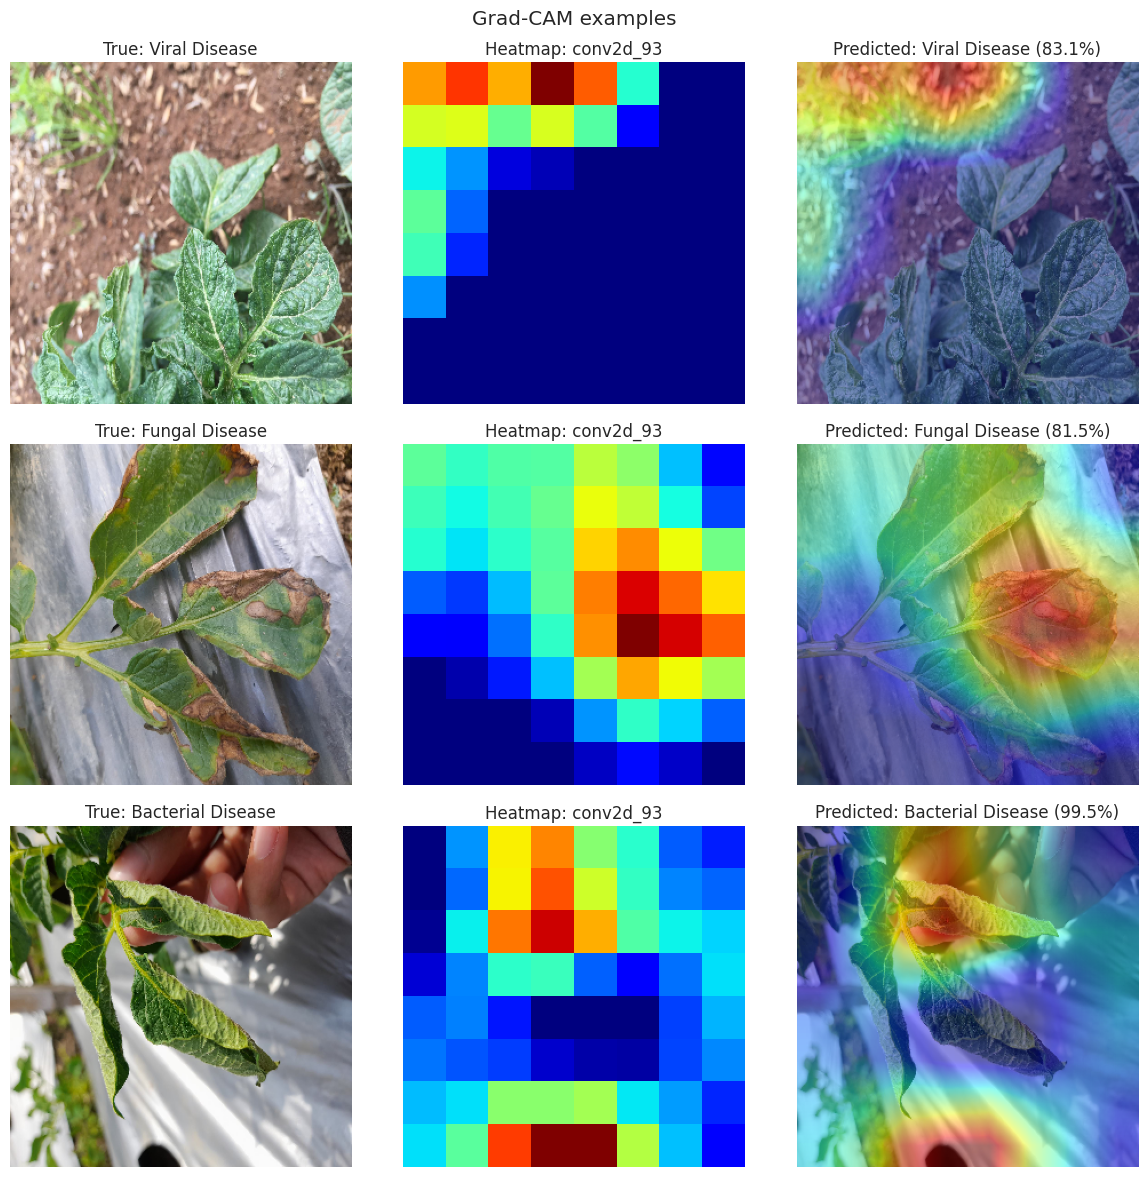
\includegraphics[width=\linewidth,height=5.4cm,keepaspectratio]{image/inception_gradcam.png}
\captionof{figure}[Grad-CAM visual explanations from the InceptionV3 benchmark.]{Grad-CAM from the InceptionV3 benchmark (\texttt{conv2d\_93}, $299 \times 299$) on the same test leaves.}
\label{fig:inception_gradcam}
\end{minipage}\hfill
\begin{minipage}[t]{0.48\textwidth}
\centering
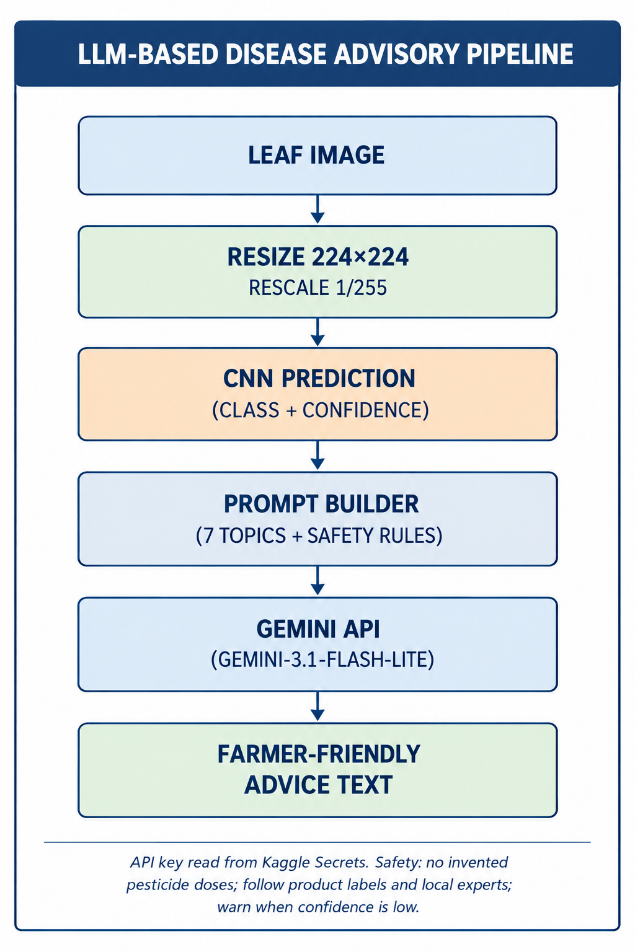
\includegraphics[width=\linewidth,height=5.4cm,keepaspectratio]{image/docx_image25.png}
\captionof{figure}[Classifier-to-LLM disease advisory workflow.]{Classifier-to-LLM advisory workflow with safety rules, from the CNN prediction to Google Gemini.}
\label{fig:llm_pipeline}
\end{minipage}
\end{figure}

\subsubsection{Web Application Deployment and Screens}
Farmers should be able to use the classifier without touching any code. So we deployed detection, Grad-CAM and Gemini advice together as a live FastAPI and React web application at \url{https://potato.mamunlab.com/}. Figures~\ref{fig:webapp_detect}--\ref{fig:webapp_info} show its five main screens.

The \textit{Detect} screen (Figure~\ref{fig:webapp_detect}) accepts a leaf photo by drag and drop (JPG/PNG up to 10~MB) or straight from the phone camera (\textit{Take a photo}). The top bar links to \textit{Detect}, \textit{Results}, \textit{Batch}, \textit{Chat} and \textit{Info}, and has switches for \textbf{English/Bengali} and \textbf{Light/Dark} mode.

The \textit{Results} screen (Figure~\ref{fig:webapp_results}) shows the predicted disease, the softmax confidence and the probability of each class. The original photo appears next to the Grad-CAM \textit{Attention overlay}. There is also an experimental attention-level indicator, with a clear note that it is not a clinical measure, and a button to download a \textbf{PDF report}.

The \textit{Batch Analysis} screen (Figure~\ref{fig:webapp_batch}) checks up to 12 leaf photos in one request, which helps when scouting a field. It counts Healthy and Diseased leaves, lists the top-3 probabilities for each leaf and exports the table with \textbf{Download CSV}.

The \textit{Disease Assistant} chat (Figure~\ref{fig:ai_assistant}) starts a Google Gemini conversation from the predicted class and confidence, in \textbf{Bengali} or \textbf{English}. The figure shows both Light and Dark themes. The assistant always adds safety notes and gives no doses.

\begin{figure}[H]
\centering
\captionsetup{font=small}
\begin{minipage}[t]{0.48\textwidth}
\centering
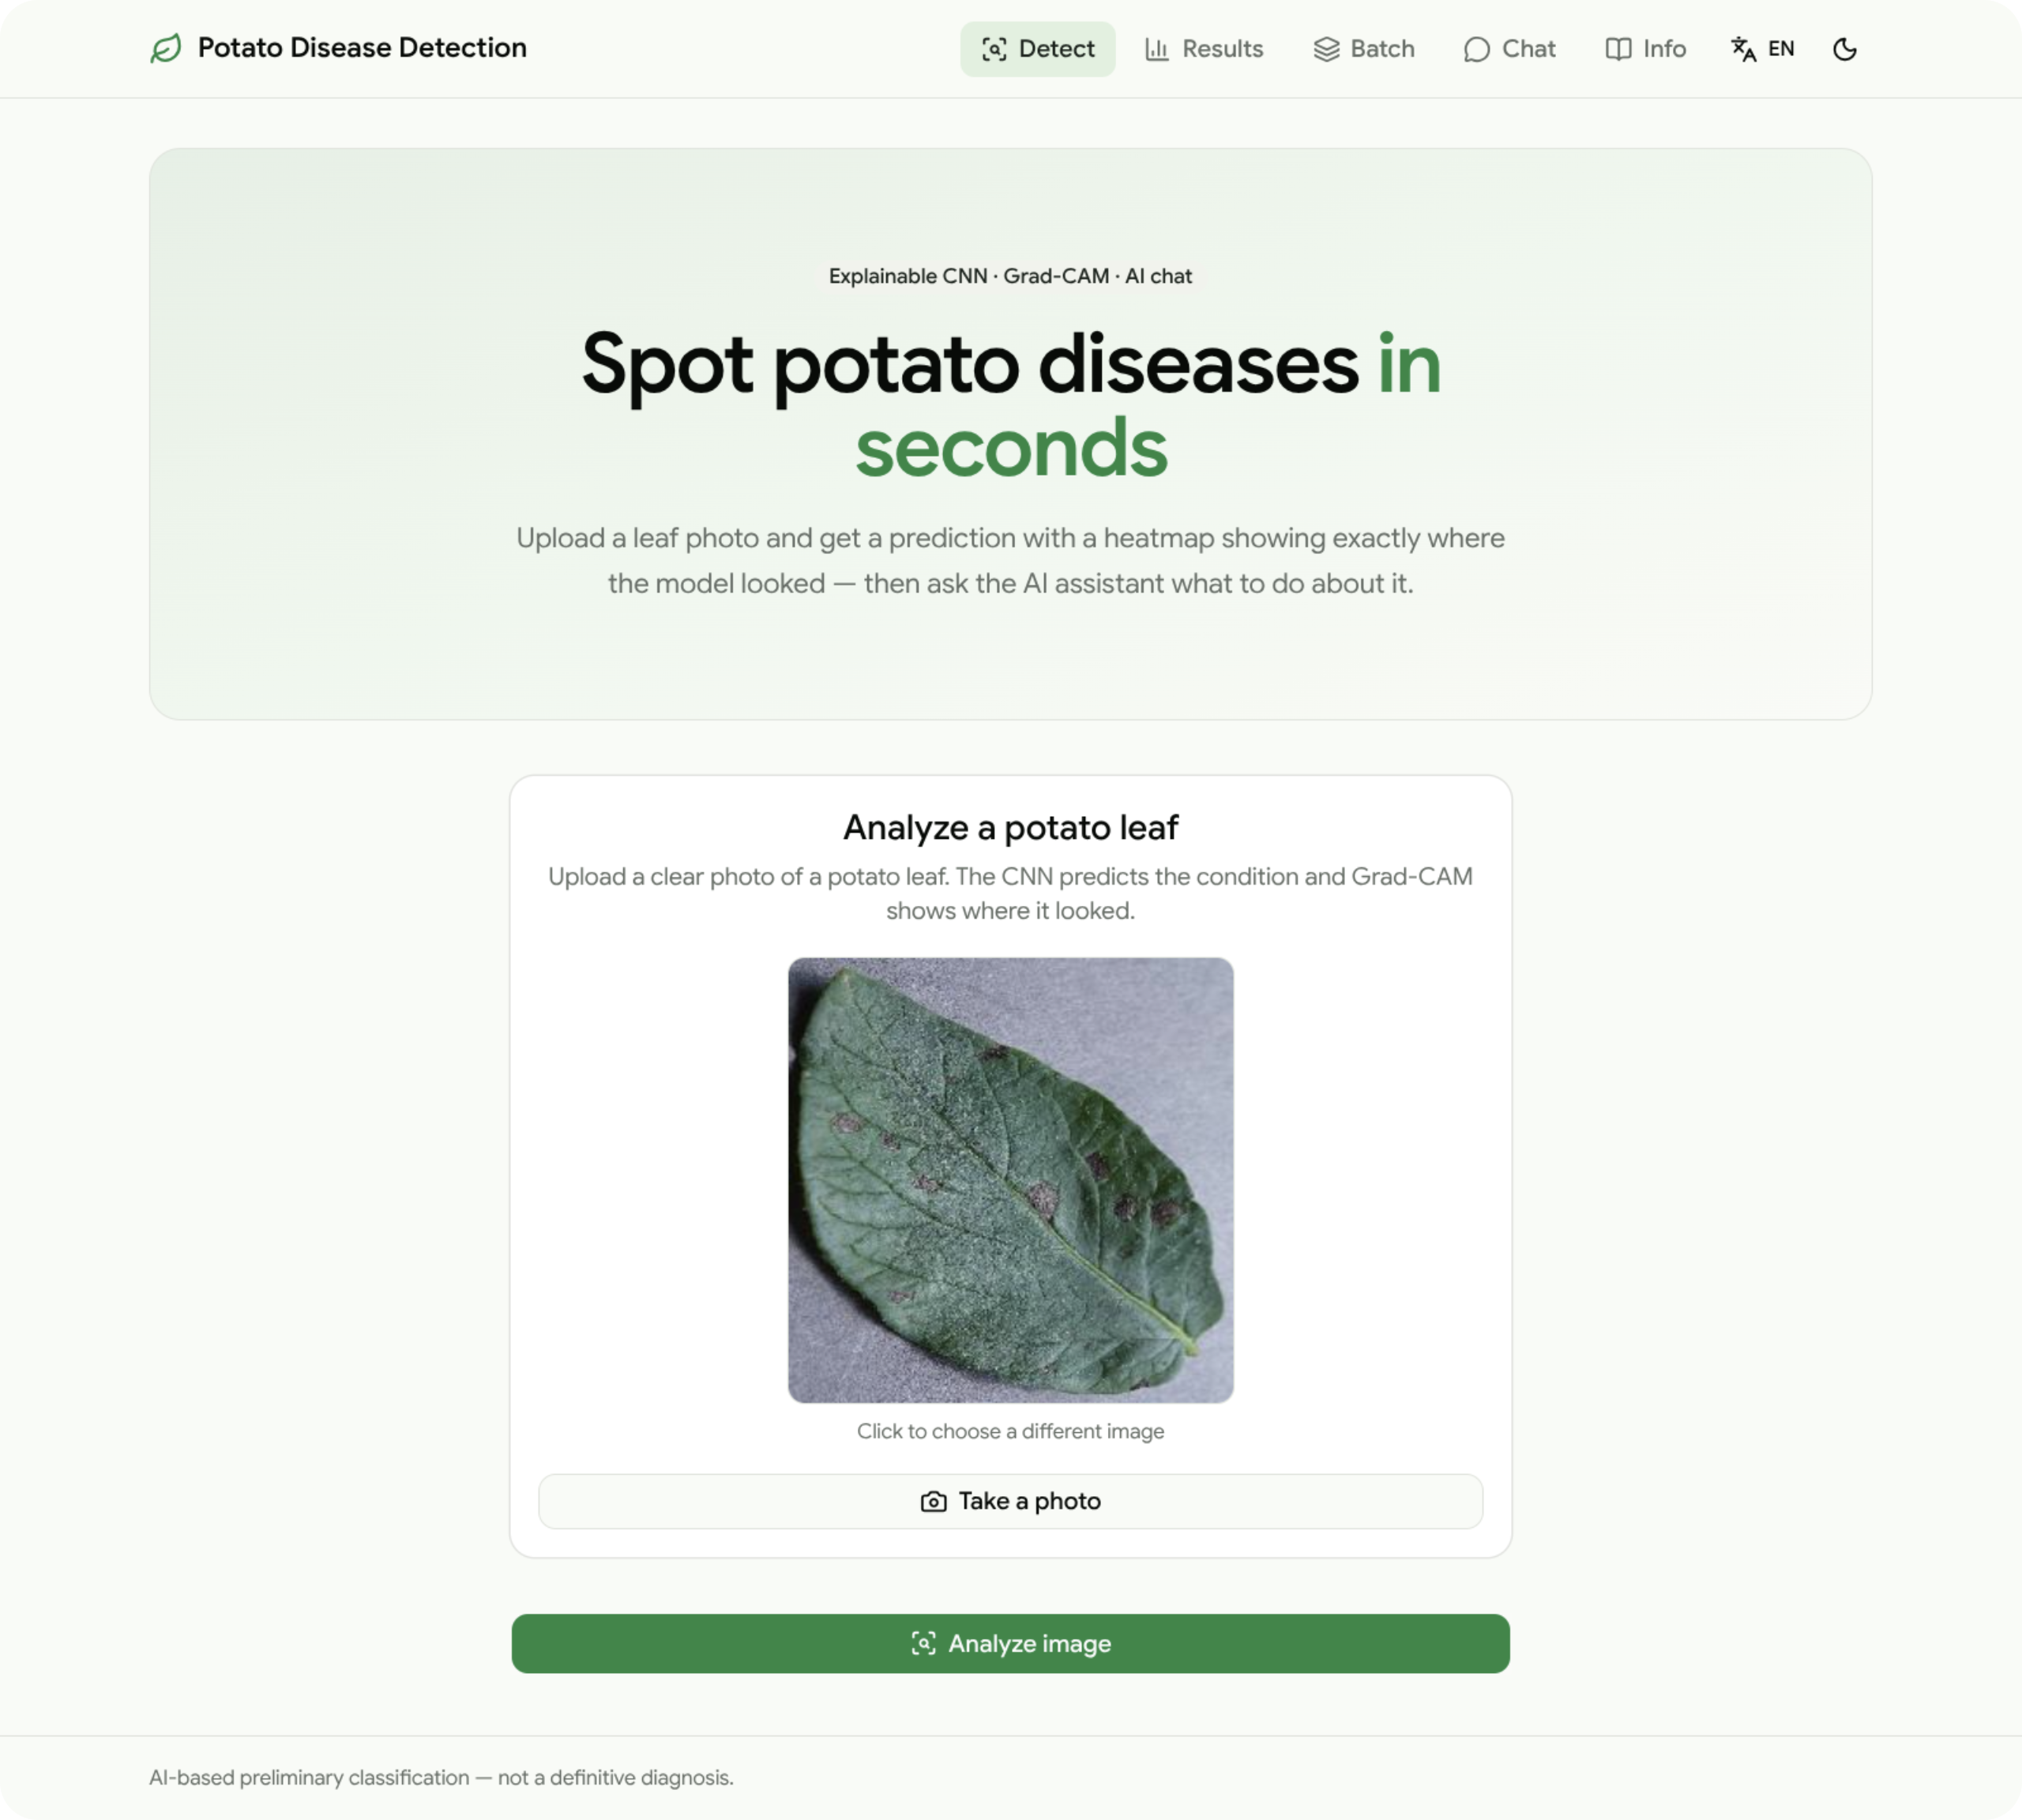
\includegraphics[width=\linewidth]{image/Select file or Take photo.png}
\captionof{figure}[Web application \textit{Detect} interface.]{\textit{Detect} page of the web app (\url{https://potato.mamunlab.com/}) with drag-and-drop upload and camera capture.}
\label{fig:webapp_detect}
\end{minipage}\hfill
\begin{minipage}[t]{0.48\textwidth}
\centering
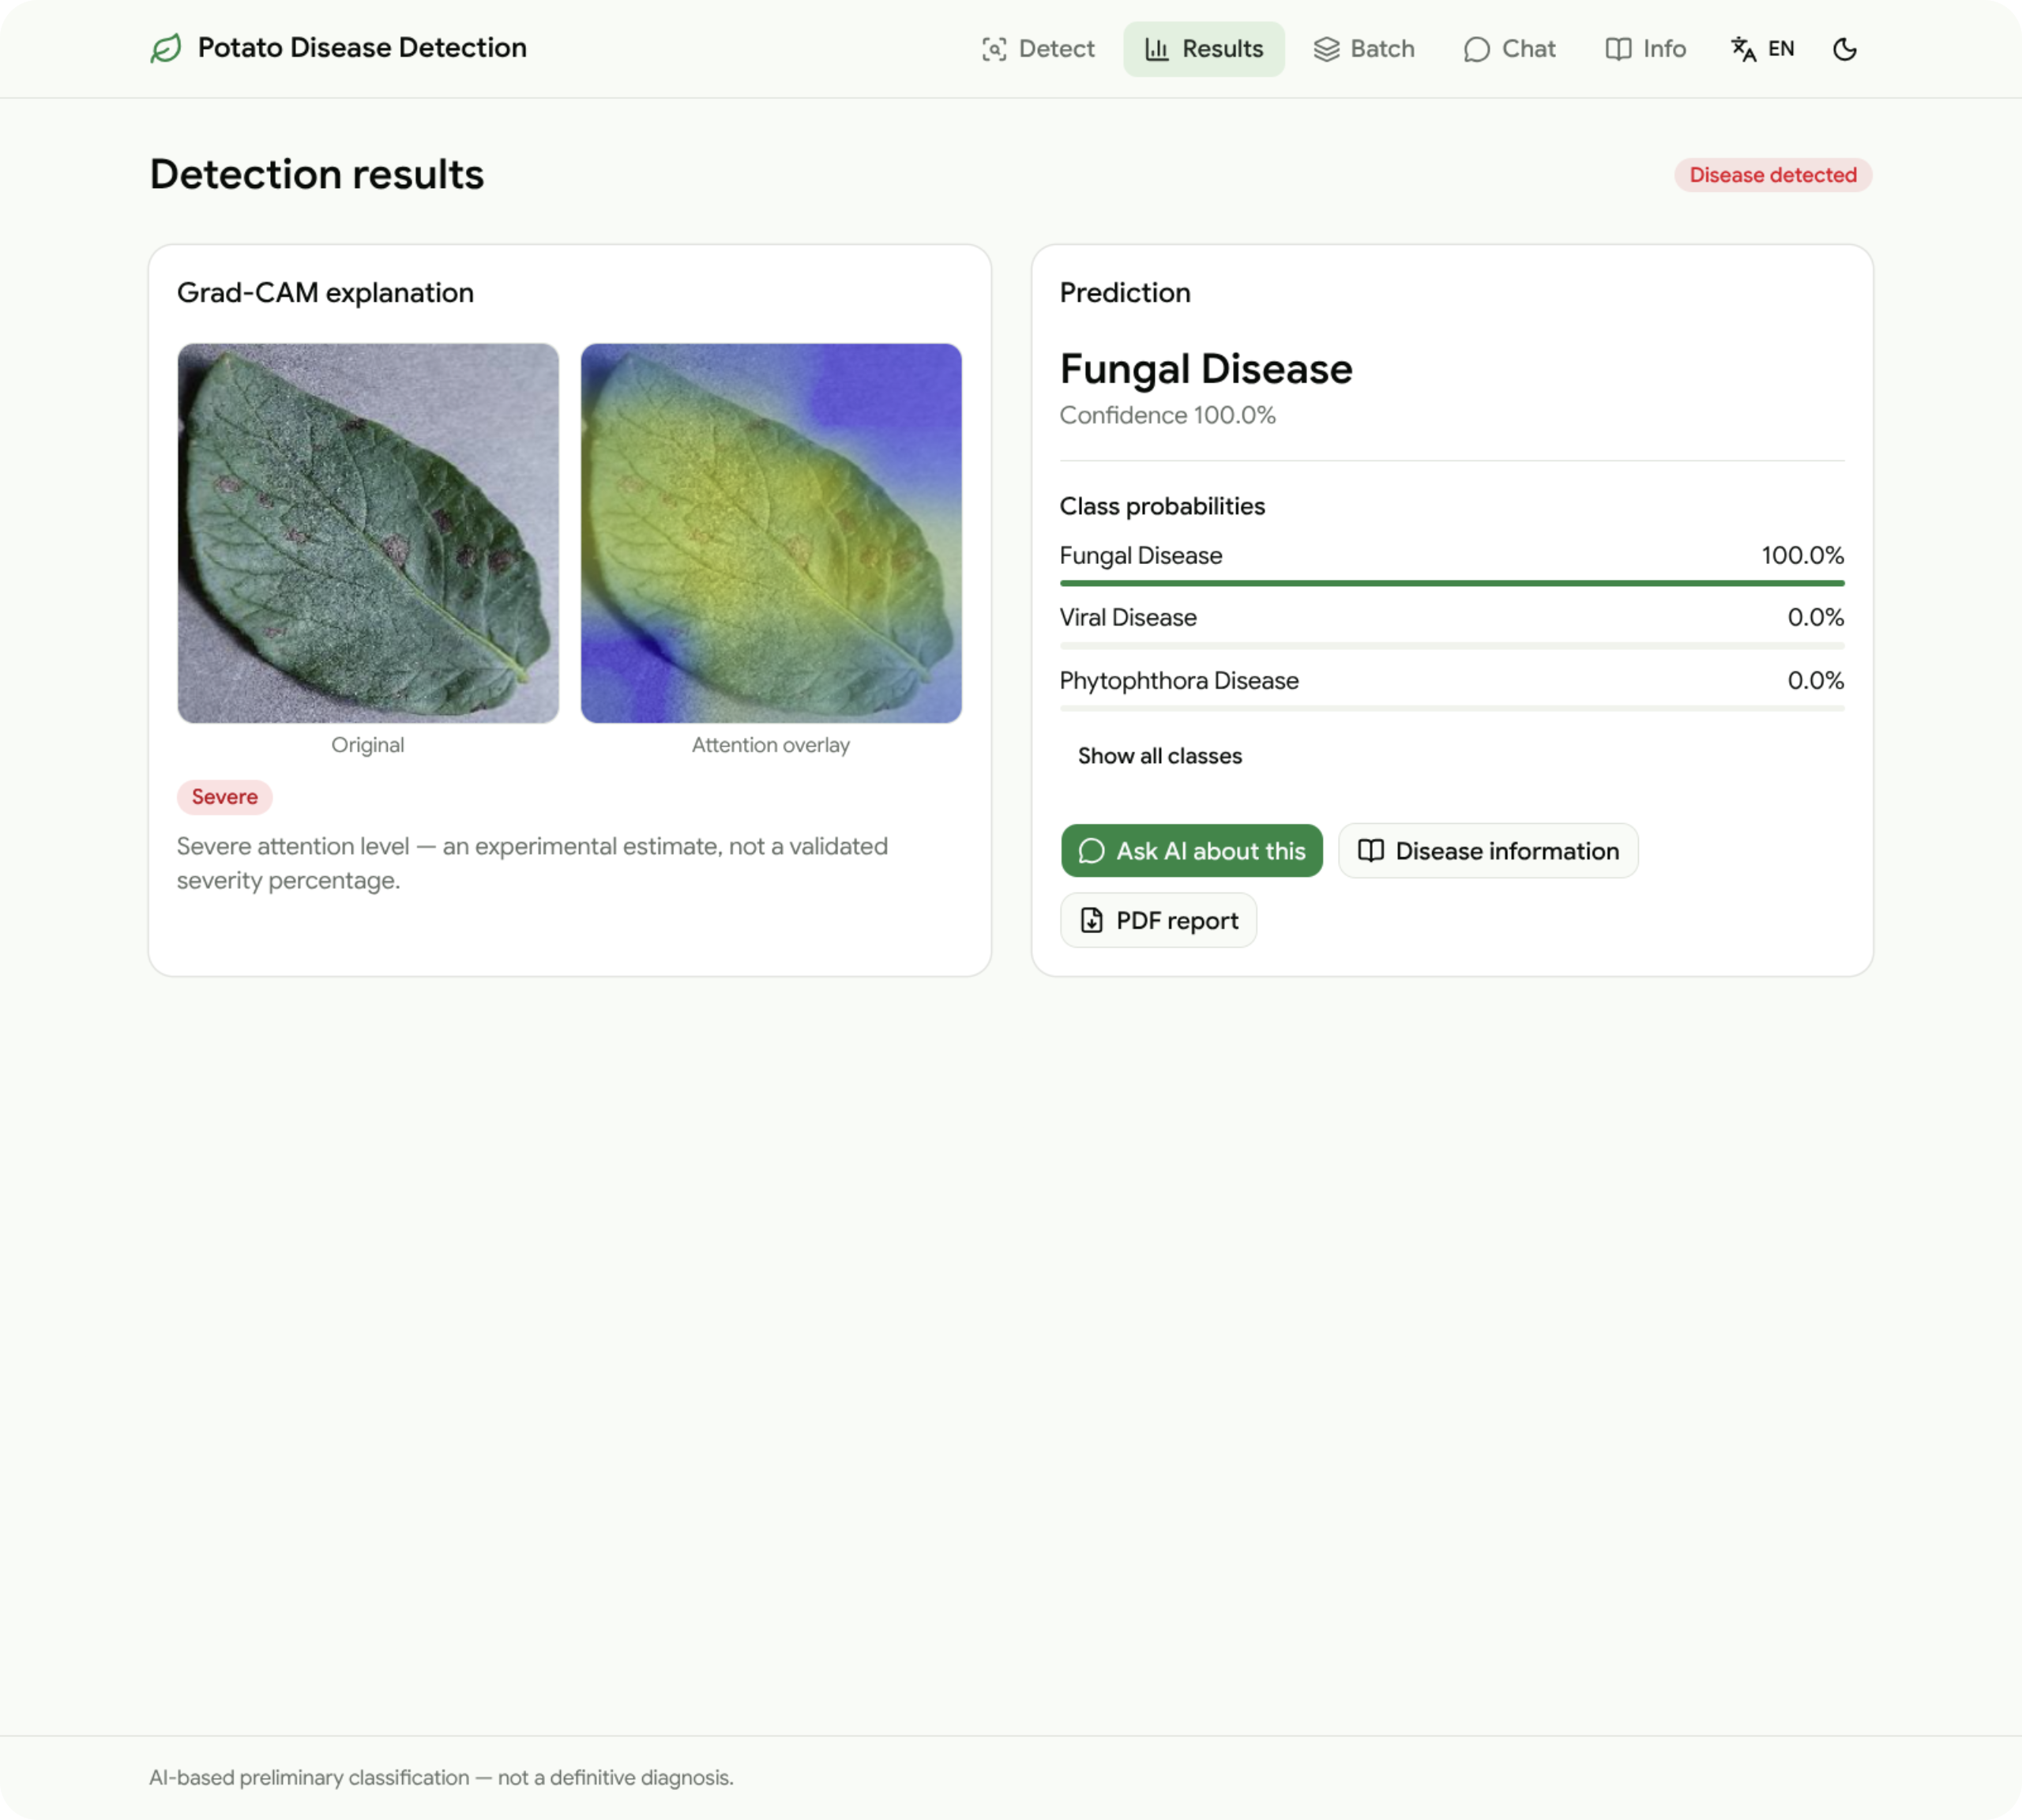
\includegraphics[width=\linewidth]{image/Detection results.png}
\captionof{figure}[Web application \textit{Results} interface.]{\textit{Results} page with the predicted class, confidence, class probabilities, Grad-CAM overlay and PDF export.}
\label{fig:webapp_results}
\end{minipage}

\vspace{6mm}

\begin{minipage}[t]{0.48\textwidth}
\centering
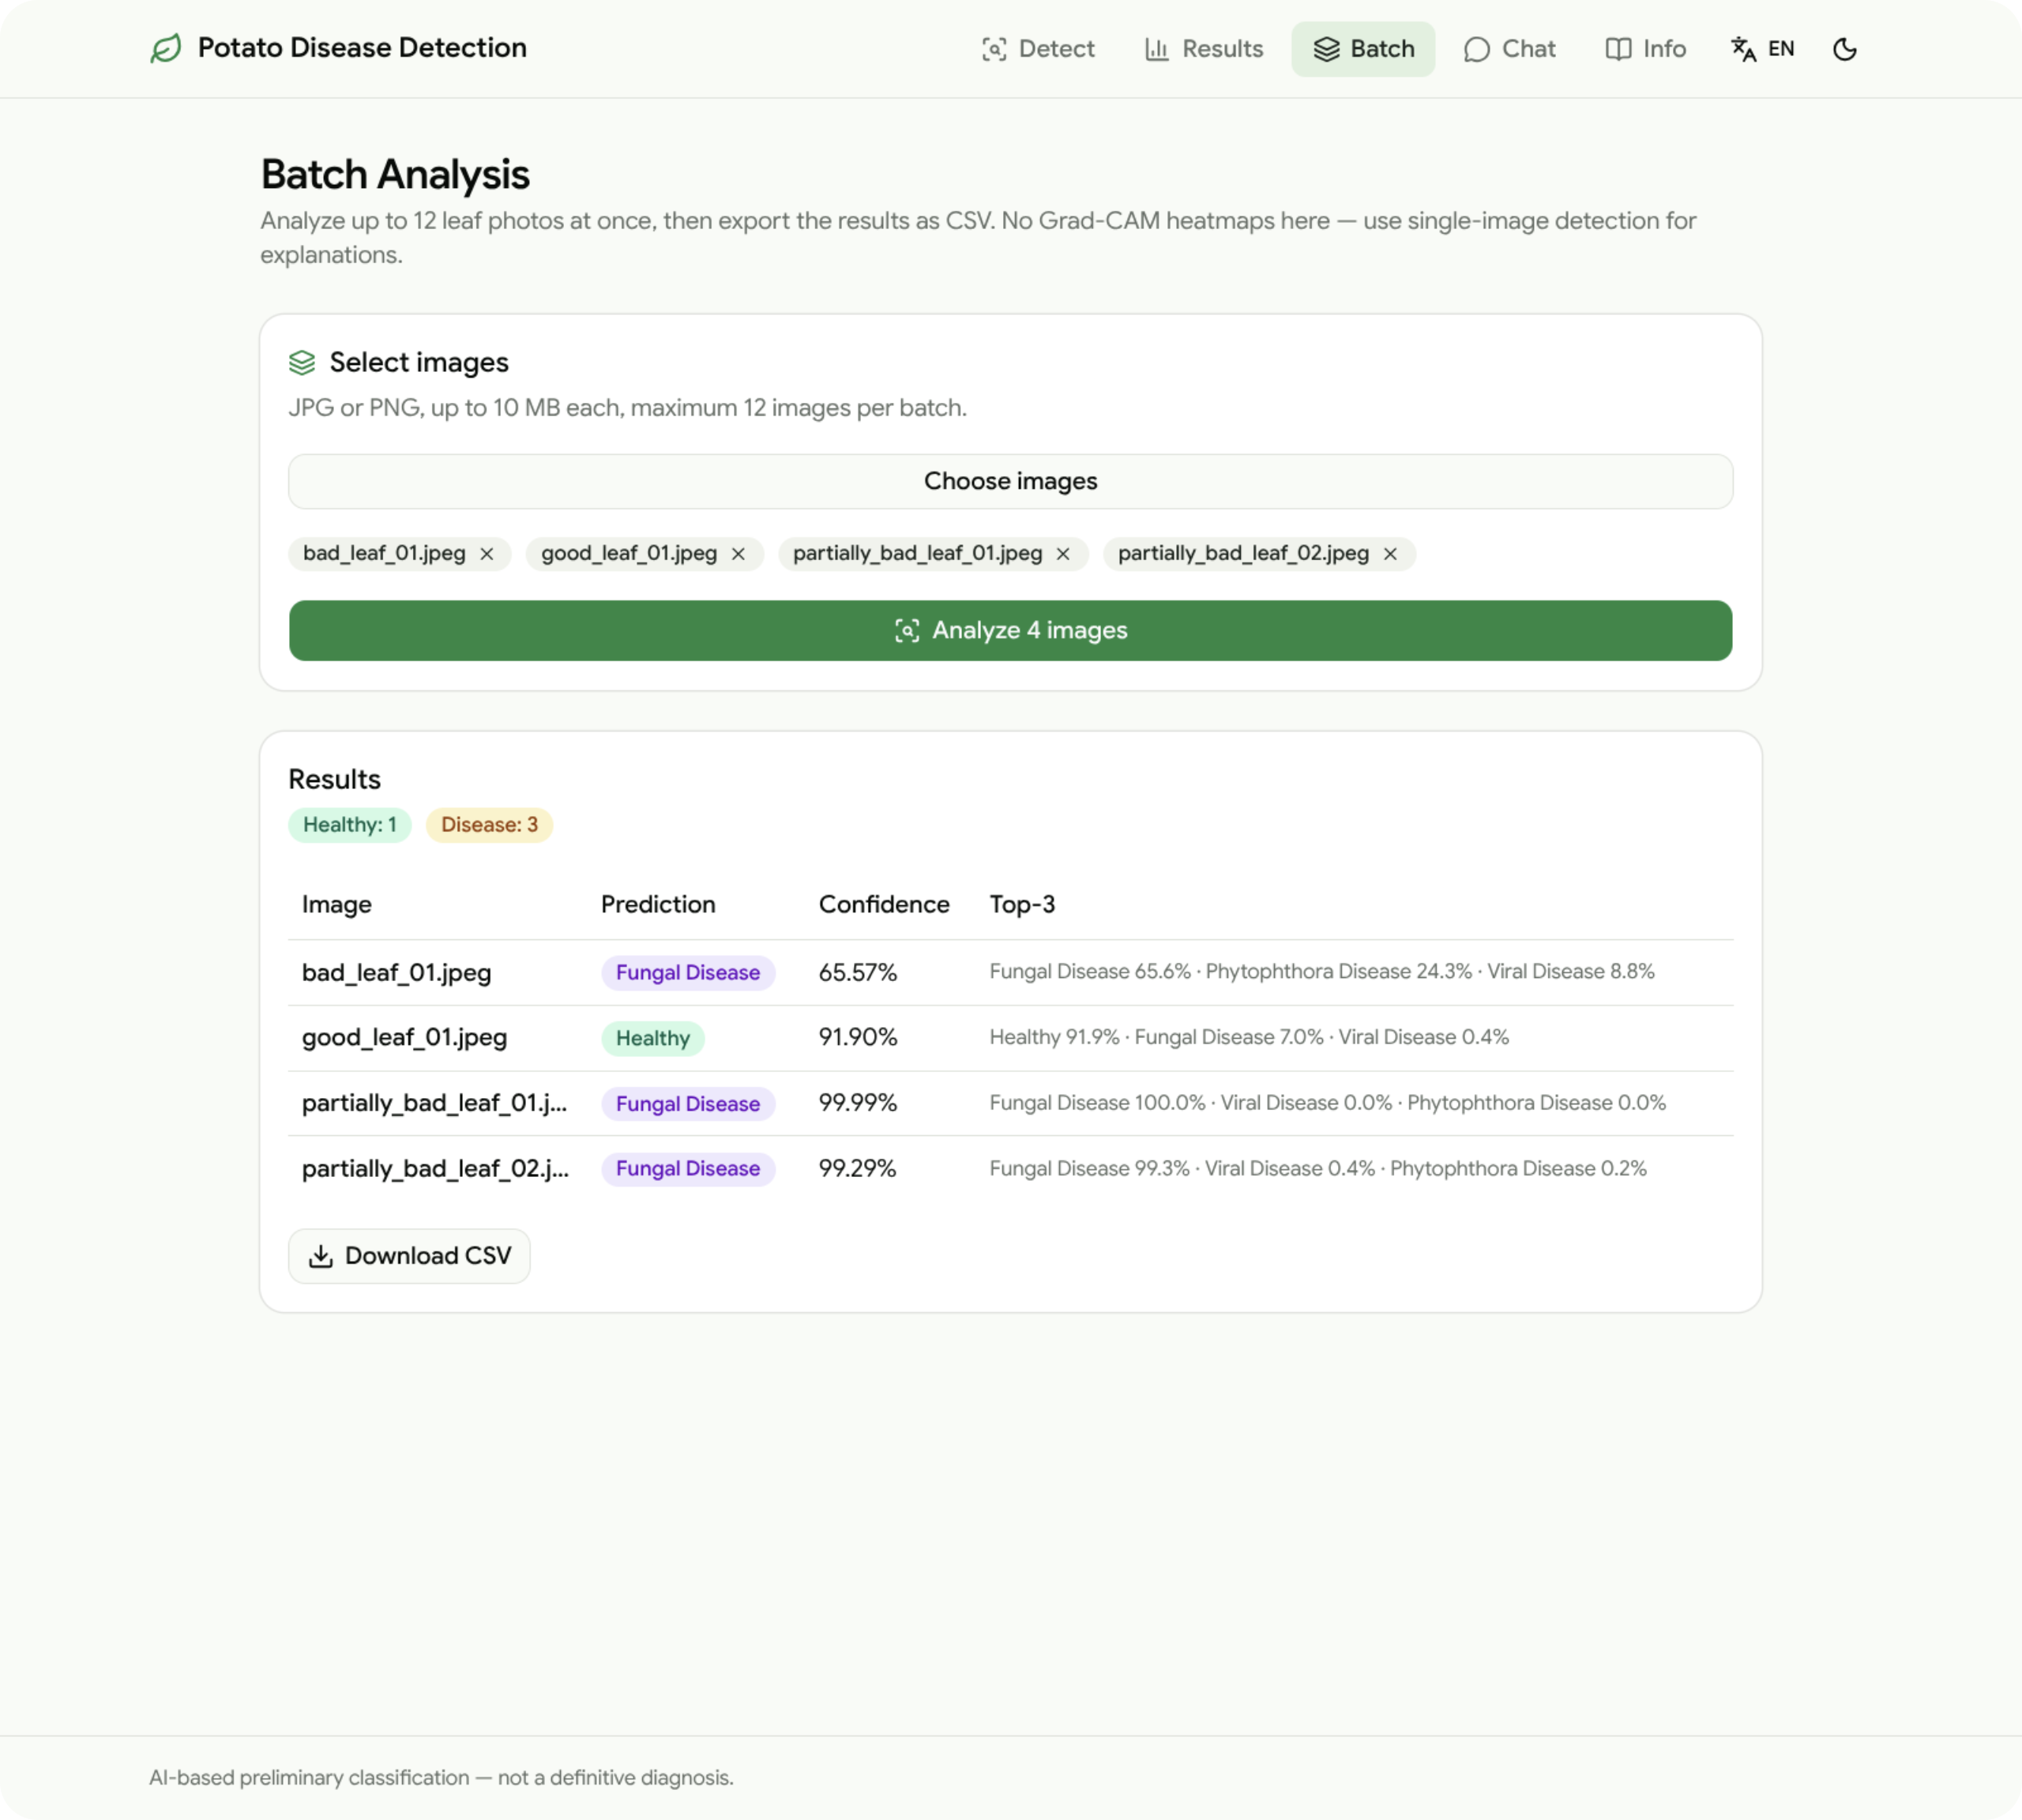
\includegraphics[width=\linewidth]{image/Batch analysis.png}
\captionof{figure}[Web application \textit{Batch Analysis} interface.]{\textit{Batch Analysis} page for up to 12 leaf photos, with Healthy/Diseased totals, top-3 probabilities and CSV export.}
\label{fig:webapp_batch}
\end{minipage}\hfill
\begin{minipage}[t]{0.48\textwidth}
\centering
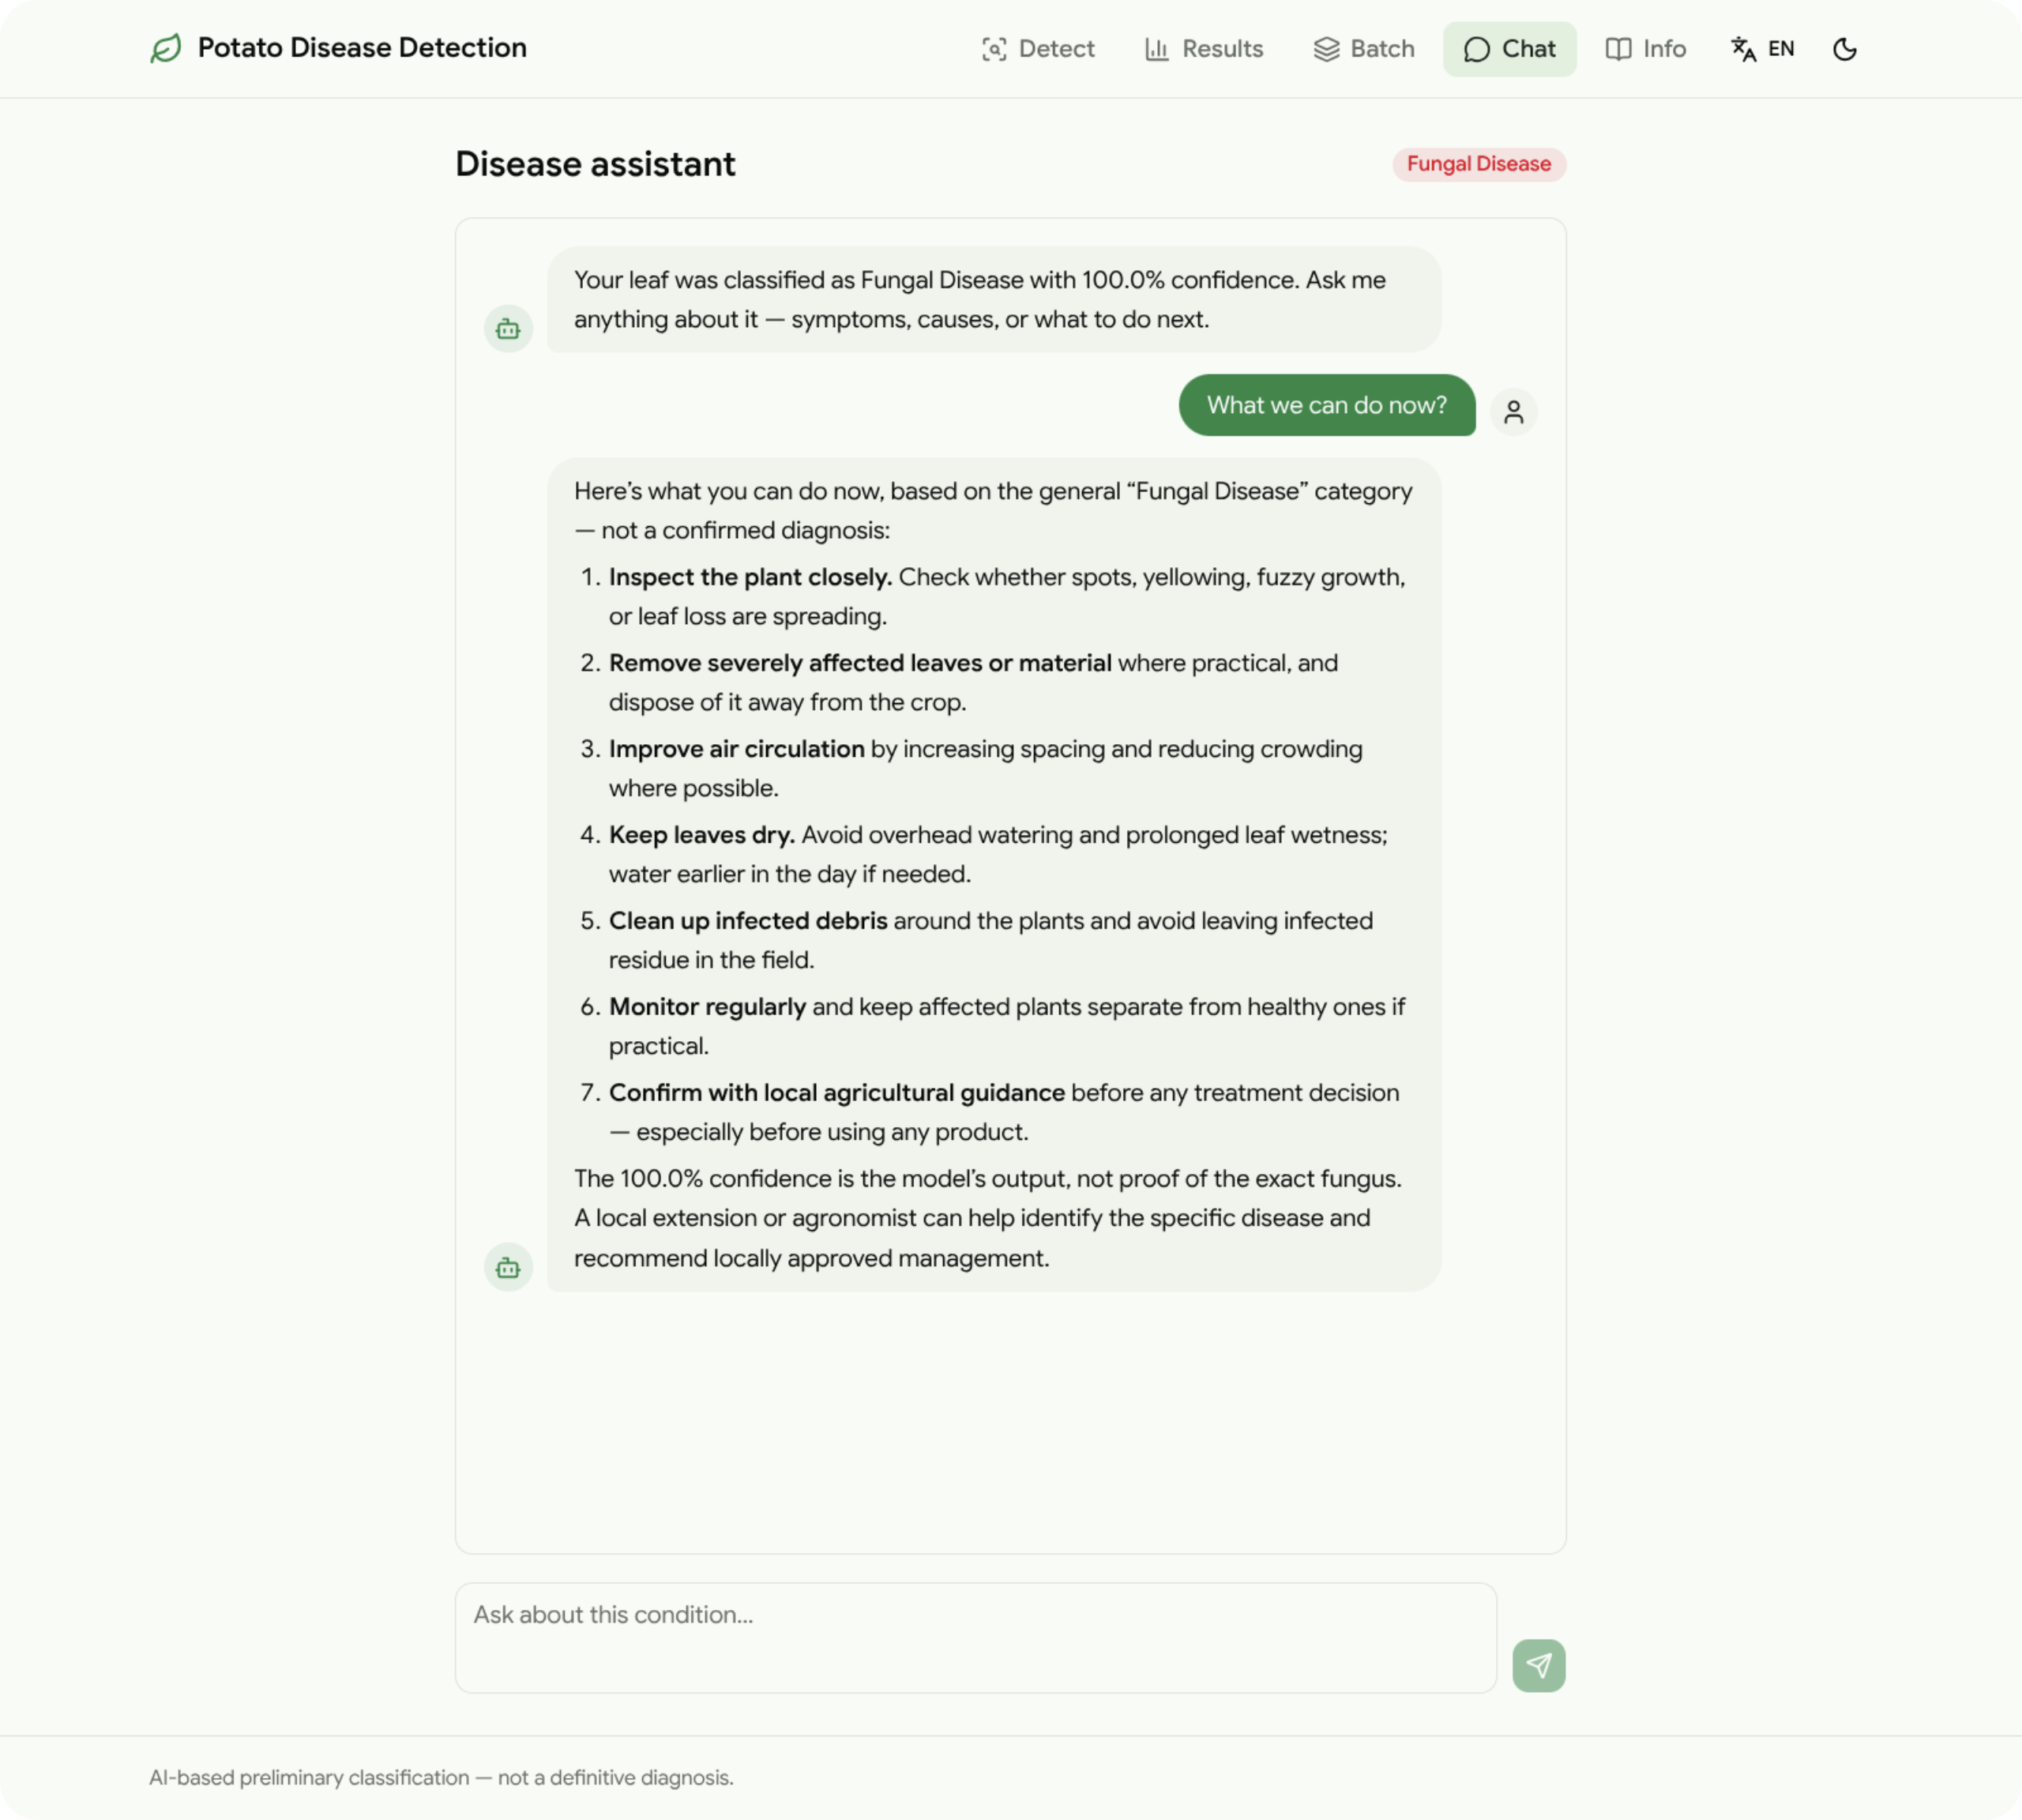
\includegraphics[width=\linewidth]{image/Disease assistant - LLM.png}
\captionof{figure}[Bilingual \textit{Disease Assistant} chat interface.]{\textit{Disease Assistant} chat in Bengali and English (Light and Dark modes), powered by Google Gemini.}
\label{fig:ai_assistant}
\end{minipage}
\end{figure}

The \textit{Info} screen (Figure~\ref{fig:webapp_info}) puts the advice on five cards: \textit{Overview}, \textit{Symptoms}, \textit{Possible causes}, \textit{Recommended actions} and \textit{Prevention}. The figure shows the cards for \textit{Fungal Disease}. Each card has a short title and a few bullet points in plain words, so a farmer can read it quickly. An \textit{Ask AI about this} button opens the chat, and a notice at the bottom says that this is only a first screening, not a final diagnosis.

\begin{figure}[!htbp]
\centering
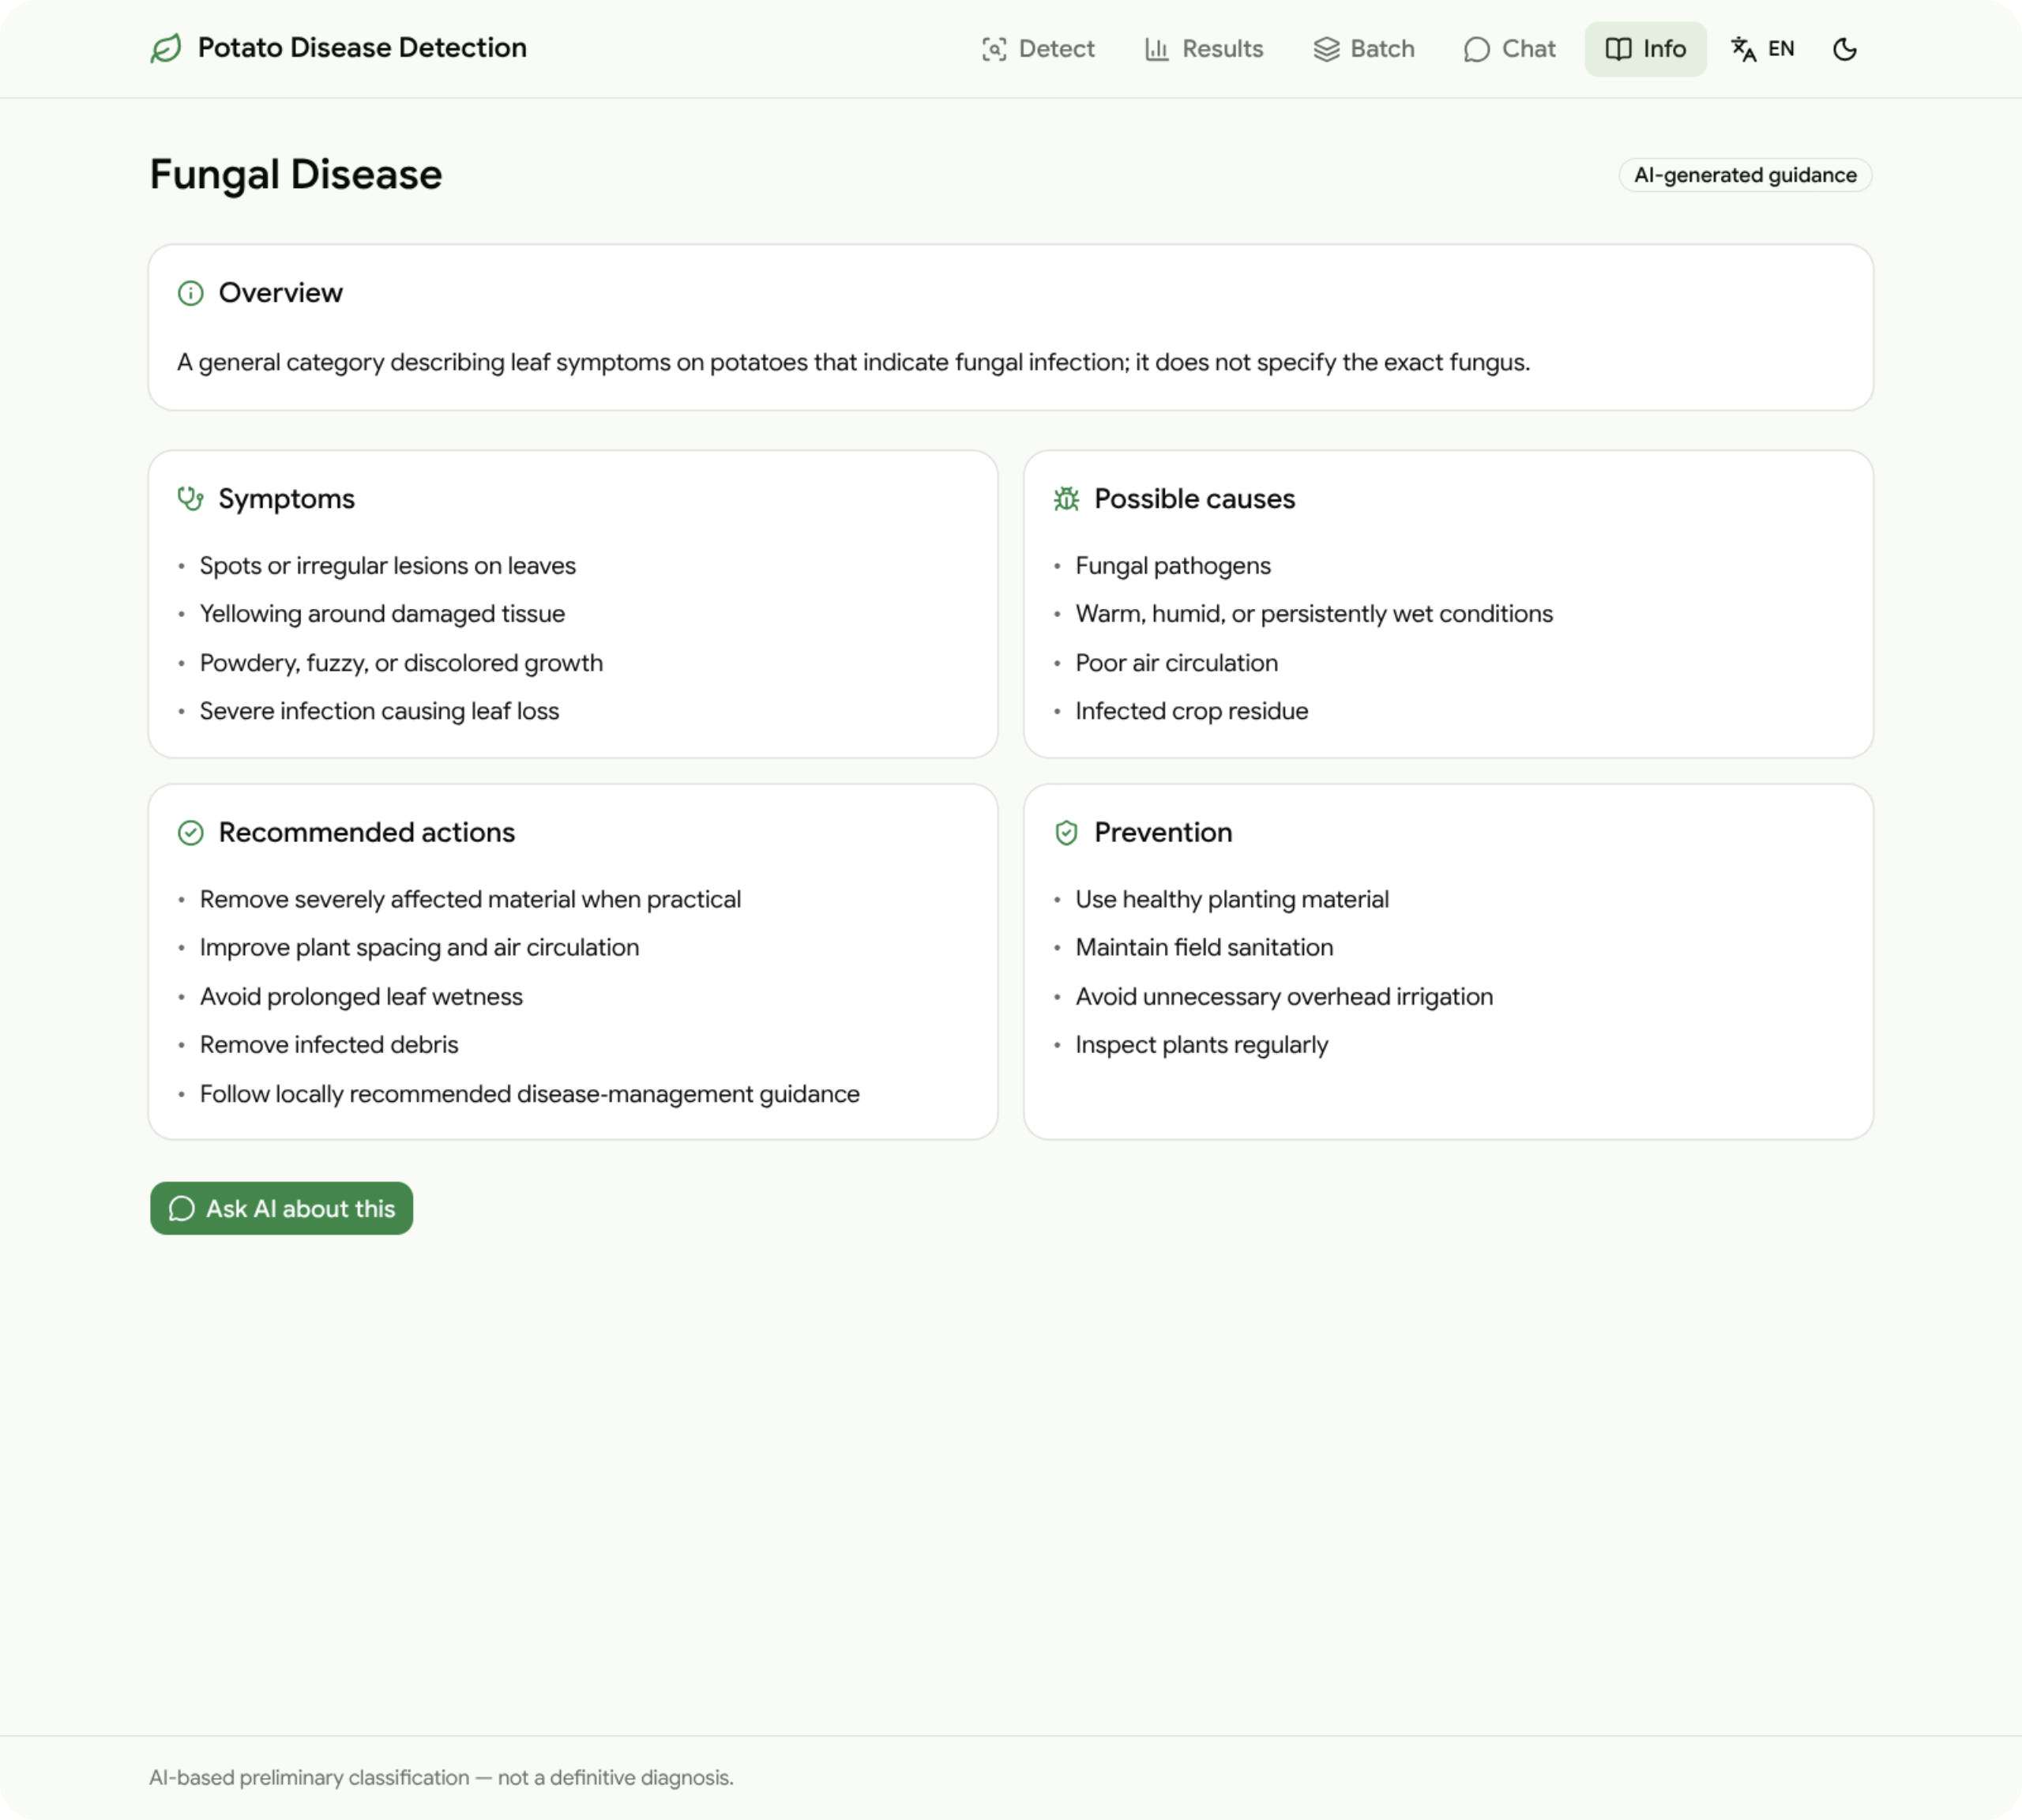
\includegraphics[width=0.55\textwidth]{image/Disease overview.png}
\caption[Web application \textit{Info} interface.]{Structured \textit{Info} view providing Overview, Symptoms, Possible causes, Recommended actions, and Prevention cards for farmers.}
\label{fig:webapp_info}
\end{figure}

\subsection{Comparison with State of the Art Model}
Table~\ref{tab:sota_comp} places our MobileNetV2 next to well-known plant disease studies and next to our own large ensemble. The PlantVillage lab studies (Mohanty et al.\ \cite{mohanty2016using}, Ferentinos \cite{ferentinos2018deep}, Too et al.\ \cite{too2019comparative}) report more than 99\% accuracy on plain backgrounds, with models of up to $\sim 138$M parameters. On cluttered outdoor photos, accuracy falls sharply \cite{mohanty2016using, shabrina2024novel}. These numbers are therefore not directly comparable with ours. On our leak-aware field benchmark, our MobileNetV2 reaches \textbf{93.51\% single-pass accuracy} (\textbf{93.94\% with 4-view TTA}, \textbf{0.9317 macro-F1}) with only \textbf{2.26M parameters (8.64~MB)}. That is about $61\times$ smaller than VGG16 and $13.7\times$ smaller than our MultiNet-V3 ensemble. Among the studies in the table, it is also the only one that combines checked Grad-CAM explanations, Gemini advice in two languages with safety rules, and a live web application for farmers.

\begin{table}[htbp]
\caption{Comparison of the Proposed MobileNetV2 System with State-of-the-Art Studies and Internal Benchmarks}
\label{tab:sota_comp}
\begin{center}
\small
\setlength{\tabcolsep}{3.5pt}
\begin{tabularx}{\textwidth}{| L{2.5cm} | L{2.2cm} | L{2.1cm} | X | L{1.6cm} | c | c |}
\hline
\textbf{Study / Model} & \textbf{Dataset / Setting} & \textbf{Architecture} & \textbf{Reported Outcome} & \textbf{Scale} & \textbf{XAI} & \textbf{App/LLM} \\
\hline
Mohanty et al.\ (2016) \cite{mohanty2016using} & PlantVillage (Lab, plain bg) & AlexNet, GoogLeNet & $>99\%$ lab (drops on field) & Heavy CNNs & No & No \\
\hline
Ferentinos (2018) \cite{ferentinos2018deep} & PlantVillage (58 classes) & VGG16 & 99.53\% (lab) & $\sim 138$M & No & No \\
\hline
Too et al.\ (2019) \cite{too2019comparative} & PlantVillage (fine-tuning) & DenseNet-121, ResNet & DenseNet-121 best (lab) & Moderate--Heavy & No & No \\
\hline
Shabrina et al.\ (2024) \cite{shabrina2024novel} & Uncontrolled Potato Field & Field benchmark & Establishes cluttered field set & Standard CNNs & No & No \\
\hline
Internal Benchmark: MultiNet-V3 & Uncontrolled Potato (5 cls, leak-aware) & EffNetB0 + MNv2 + ResNet50 & 90.91\% (0.8975 F1) & 31.08M (118.55~MB) & Yes & No \\
\hline
\textbf{Proposed MobileNetV2} & \textbf{Uncontrolled Potato (5 cls, leak-aware)} & \textbf{MobileNetV2 (Frozen-BN AdamW)} & \textbf{93.51\% / 93.94\% TTA (0.9317 F1)} & \textbf{2.26M (8.64~MB)} & \textbf{Yes} & \textbf{Yes} \\
\hline
\end{tabularx}
\end{center}
\end{table}
